\documentclass[11pt,a4paper,twoside,openright]{memoir}

%%%%%%%%%%%%%%%%%%%%%%%%%%%%%%%%%%%%%%%%%%%%%%%%%%%%%%%
%  In my opinion (DW) there are no fonts available in the standard
%  TeX/LaTeX set that are ideal for this use, unless you go down to 9pt or 
%  8pt for your text face, and this is too small.  If you have Metafont you
%  should consider generating a cmr17 font at a magstep of two (about 25pt)
%  or three (about 30pt), or even more, depending on the point size of your
%  main text.  Why not go the whole hog and design some really fancy 
%  capitals from scratch!
%
%%%%%%%%%%%%%%%%%%%%% BOX ONE %%%%%%%%%%%%%%%%%%%%%%%%%
%\typein[\dropinitialfont]{Font for Dropped initial:} %
%\font\largefont \dropinitialfont                     %
%%%%%%%%%%%%%%%%%%%%%%%%%%%%%%%%%%%%%%%%%%%%%%%%%%%%%%%
%
%%%%%%%%%%%%%%%%%%%%% BOX TWO %%%%%%%%%%%%%%%%%%%%%%%%%
%\font\largefont= cmr10 scaled \magstep5              %
%\font\largefont= cmbx10 scaled \magstep5             %
%\font\largefont= cmbx17 scaled \magstep3             %
\font\largefont= cmr17 scaled \magstep5               %
%%%%%%%%%%%%%%%%%%%%%%%%%%%%%%%%%%%%%%%%%%%%%%%%%%%%%%%

% Copyright Symbole u..
\def\TReg{\textsuperscript{\textregistered}}
\def\TCop{\textsuperscript{\textcopyright}}
\def\TTra{\textsuperscript{\texttrademark}}

\def\drop#1#2{{\noindent
    \setbox0\hbox{\largefont #1}\setbox1\hbox{#2}\setbox2\hbox{(}%
    \count0=\ht0\advance\count0 by\dp0\count1\baselineskip
    \advance\count0 by-\ht1\advance\count0by\ht2
    \dimen1=.5ex\advance\count0by\dimen1\divide\count0 by\count1
    \advance\count0 by1\dimen0\wd0
    \advance\dimen0 by.25em\dimen1=\ht0\advance\dimen1 by-\ht1
    \global\hangindent\dimen0\global\hangafter-\count0
    \hskip-\dimen0\setbox0\hbox to\dimen0{\raise-\dimen1\box0\hss}%
    \dp0=0in\ht0=0in\box0}#2}

% end of new \drop command
%%%%%%%%%%%%%%%%%%%%%%%%%%%%%%%%%%%%%%%%%%%%%%%%%%%%%%%

%%%%%%%%%%%%%%%%%%%%%%%%%%%%%%%%%%%%%%%%%%%%%%%%%%%%%%%
% new \versal command
\newcommand{\versal}[1]{{\noindent
    \setbox0\hbox{\largefont #1}%
    \count0=\ht0                   % height of versal
    \count1=\baselineskip          % baselineskip
    \divide\count0 by \count1      % versal height/baselineskip
    \dimen1 = \count0\baselineskip % distance to drop versal
    \advance\count0 by 1\relax     % no of indented lines
    \dimen0=\wd0                   % width of versal
    \global\hangindent\dimen0      % set indentation distance
    \global\hangafter-\count0      % set no of indented lines
    \hskip-\dimen0\setbox0\hbox to\dimen0{\raise-\dimen1\box0\hss}%
    \dp0=0in\ht0=0in\box0}}
% end of new \versal command
%%%%%%%%%%%%%%%%%%%%%%%%%%%%%%%%%%%%%%%%%%%%%%%


%%%%%%%%%%%%%%%%%%%%%%%%%%%%%%%%%%%%%%%%%%%%%%%
% redefining the textblocksize
%%%%%%%%%%%%%%%%%%%%%%%%%%%%%%%%%%%%%%%%%%%%%%%
\setlrmarginsandblock{1in}{1.5in}{*}
\checkandfixthelayout
%%%%%%%%%%%%%%%%%%%%%%%%%%%%%%%%%%%%%%%%%%%%%%%


\usepackage{graphicx}
\usepackage{latexsym}
\usepackage{epsfig}
\usepackage[figuresright]{rotating}
\usepackage{dsfont}
\usepackage{german}
\usepackage[utf8]{inputenc}
%\usepackage[dvips]{color}
\usepackage{colortbl}
	\definecolor{darkblue}{rgb}{0,0,0.4}
	\definecolor{darkgray}{rgb}{0.1,0.1,0.2}
	\definecolor{darkred}{rgb}{0.6,0.0,0.0}
   \definecolor{darkgreen}{rgb}{0.0,0.6,0.0}
   \definecolor{orange}{rgb}{1.0,0.8,0.0}

%---- for algorithms ----
\usepackage[Algorithmus]{algorithm}
\usepackage{algorithmic}

%---- for the index ----
\usepackage{layouts}[2001/04/29]
\makeindex

\usepackage{hyperref}
\usepackage{memhfixc}
\hypersetup{colorlinks=true,linkcolor=darkgray,urlcolor=darkblue,citecolor=darkblue,filecolor=darkgreen}

%---- a second bibliography ----
\usepackage{multibib}
\renewcommand{\refname}{Allgemeine Literaturquellen}

%---- some new math symbols ----
\usepackage{nicefrac} % schräge bruchstriche
\usepackage{amssymb}
\newcommand{\Real}{\mathbb R}

%---- memoir package specialties
%\pagestyle{companion}
\pagestyle{Ruled}
\setlength{\epigraphwidth}{7cm}
\setcounter{tocdepth}{3}
\setcounter{secnumdepth}{3}
\maxsecnumdepth{subsection}

% change standard font
%\usepackage{cmbright}
\renewcommand{\rmdefault}{cmss}
\renewcommand{\sfdefault}{cmss}

% set figure resp. table name and number bold
\makeatletter
\renewcommand{\fnum@figure}{\textbf{\figurename~\thefigure}}
\renewcommand{\fnum@table}{\textbf{\tablename~\thetable}}
\makeatother

% setting the authors for a verse
\newcommand{\attrib}[1]{%
	\nopagebreak{\raggedleft\footnotesize #1\par}}

%---- general information ----
\author{ 
	\small{vorgelegt von} \vspace{.5cm} 											\\ 
	\Large{\textbf{Lukas Michael Müller}} 											\\ 
	\small{geb.\ in Schotten}}
\title{
	\textbf{\vspace{-2.5cm}
		%--------------------------------------------------------------
		% unter mac os x können Sie auch ein .png als Bild einbinden...
		%--------------------------------------------------------------
		\includegraphics[width=16.0cm]{logo_thm_cf_4c.png} \\
		\vspace{3cm} Technologieanalyse mit Angular und WebGL zur Umsetzung eines Konfigurators für Mehrwegbecher} \\
	\vspace{1cm}
	\normalsize{Studiengang Medieninformatik} \vspace{1cm} \\
	\Large{\textbf{Bachelorarbeit}} }
\date{}


\begin{document}
	%---- the frontmatter ----
	\frontmatter
	
		\begin{titlingpage}
			\begin{center}
				%---- create the title page ----
				\maketitle
				\vspace{-1cm}
				\small{durchgeführt in bei} \\
				\small{Yellow Tree - Agentur für Kommunikation \& Design, Siegen}
				\begin{tabular}{ll}
					& \\
					& \\
					& \\
					Referent der Arbeit: & Prof. Dr. Benjamin Einert \\
					Korreferent der Arbeit: & Prof. Dr. Stefan Euler \\
					Betreuer bei Yellow Tree: & Dipl.-Ing. Andreas Utsch \\
					& \\
				\end{tabular}
				
				\vspace{\fill}
				\small{Friedberg, 2019}
			\end{center}
			
		\end{titlingpage}
	
	%---- Widmung ----
	\thispagestyle{empty}
	\begin{flushright}
		\vspace*{\fill}
		\Large{\textsl{\rmfamily{F"ur Yellow Tree}}}
		\vspace{15cm}
	\end{flushright}

	\cleardoublepage
	\setcounter{page}{1}
	
	%---- Danksagung ----
	\chapter{Danksagung}
Normalerweise haben eine ganze Reihe von Personen mehr oder wenig Anteil am Gelingen der Bachelorarbeit, denen man hier dankt: In der Regel zunächst den Referenten und Betreuern der Arbeit. Aber natürlich auch Personen, Firmen und Institutionen, die die Arbeit tatkräftig unterstützt haben. Sei es durch die Bereitstellung von spezieller Hard- oder Software oder nur durch ein gewissenhaftes Korrekturlesen.
\\


	%---- Selbststädigkeitserkläung ----
	\chapter{Selbstständigkeitserklärung}
\label{cha:erklaerung}
%
%
Ich erkläre, dass ich die eingereichte Bachelorarbeit selbstständig und ohne fremde Hilfe verfasst, andere als die von mir angegebenen Quellen und Hilfsmittel nicht benutzt und die den benutzten Werken wörtlich oder inhaltlich entnommenen Stellen als solche kenntlich gemacht habe. \\
%
\vspace{.2cm} \\
\noindent Friedberg, Monat 2014 \\
%
\vspace{2cm} \\
\noindent Kevin-Horst Bratzke \\
%
%
%

	
	\cleardoublepage
	
	%---- table of contents ----
	\tableofcontents
	
	\cleardoublepage
	
	%---- list of figures ----
	\listoffigures
	
	%---- the mainmatter ----
	\mainmatter

		%---- Einführung ----
		%
%%%%%%%%%%%%%%%%%%%%%%%%%%%%%%%%%%%%%%%%%%%%%%%%%%%
%
% E I N L E I T U N G
%
%%%%%%%%%%%%%%%%%%%%%%%%%%%%%%%%%%%%%%%%%%%%%%%%%%%
%
\chapter{Einleitung}
\label{cha:introduction}
%
%
Mit dem folgenden Kapitel soll eine Einführung in das Thema gegeben werden. Es wird darauf eingegangen, warum dieses Thema relevant ist. Außerdem wir das Problem beschrieben, sowie das Ziel festgelegt. Am Ende des Kapitels wird auf den Aufbau der Arbeit eingegangen.
%
%
%%%%%%%%%%%%%%%%%%%%%%%%%%%%%%%%%%%%%%%%%%%%%%%%%%%
%
% Motivation
%
%%%%%%%%%%%%%%%%%%%%%%%%%%%%%%%%%%%%%%%%%%%%%%%%%%%
%
\section{Motivation}
\label{sec:motivation}
%
Der Kunde \textit{Gizeh\footnote{\textbf{Gizeh Verpackungen} ist eine international tätige deutsche Unternehmensgruppe die Kunststoffverpackungen entwirft, fertigt und dekoriert. Das Unternehmen, dessen Stammsitz sich im nordrhein-westfälischen Bergneustadt befindet, beschäftigt gegenwärtig insgesamt etwa 750 Mitarbeiter und erwirtschaftete 2017 einen Umsatz von etwa 120 Millionen Euro.}} bedruckt individuelle Mehrwegbecher. Große Druckportale, wie \textit{Fyleralarm\footnote{Die \textbf{flyeralarm GmbH} ist eine Online-Druckerei mit Sitz in Würzburg. Das Unternehmen ist auf die Herstellung und den Vertrieb von Drucksachen spezialisiert. Das Druckereiunternehmen gehört zu 100 Prozent dem Gründer Thorsten Fischer und ist in 15 europäischen Ländern präsent.}}, senden ihre Aufträge an \textit{Gizeh}. Dieser produziert dann die Becher, sowie den späteren Druck. Ein webbasierter Konfigurator könnte der Firma ermöglichen zukünftig Direktbestellungen aufzunehmen. Damit hätte der Kunde eine einfache Möglichkeit sein Design in einer 3D Ansicht zu sehen und ganz einfach zu konfigurieren. So hat man bevor der Becher bestellt wird schon einmal gesehen, wie es aussehen wird. \\
Schon in anderen Branchen, wie zum Beispiel auf dem Automarkt, wird dieses Prinzip der 3D Konfiguratoren angewandt. 
%
%
%%%%%%%%%%%%%%%%%%%%%%%%%%%%%%%%%%%%%%%%%%%%%%%%%%%
%
% Problemstellung
%
%%%%%%%%%%%%%%%%%%%%%%%%%%%%%%%%%%%%%%%%%%%%%%%%%%%
%
\section{Problemstellung}
\label{sec:problemstellung}
%
Wenn man einen Mehrwegbecher beispielsweise über \textit{Flyeralarm} bedrucken lassen will, sollte ein fertiges Design vorliegen. Dabei gibt es keine speziellen Vorgaben bzgl. der kubischen Form. Man kann lediglich ein Design im \texttt{PDF}-Format hochladen. Nebenbei wird man darauf hingewiesen, das aufgrund der kubischen Form das Design gestaucht wird. Somit werden beispielsweise Kreise eventuell nicht ganz rund dargestellt. \\ 
%
Dem Kunden wäre es somit ein Vorteil, eine Vorschau des bedruckten Bechers anschauen zu können. Die Lösung könnte ein 3D Konfigurator für Mehrwegbecher sein. Es gibt schon einige 3D Konfiguratoren. Allerdings besteht bei diesem die Frage: Wie kann der designte Becher optimal dargestellt werden? Und wie kann eine eventuell notwendige Anpassung des Designs erfolgen? Gerade wenn man den Aspekt der Responsivität hinzunimmt findet man keine bestehende Lösung, die zufriedenstellend wäre. Dieser Aspekt wird in Grundlagen Kapitel 3 unter dem Punkt \ref{sec:responsive} \textit{Responsive Webdesign} genauer erläutert.
%
%
%%%%%%%%%%%%%%%%%%%%%%%%%%%%%%%%%%%%%%%%%%%%%%%%%%%
%
%  Zielsetzung
%
%%%%%%%%%%%%%%%%%%%%%%%%%%%%%%%%%%%%%%%%%%%%%%%%%%%
%
\section{Zielsetzung}
\label{sec:zielsetzung}
%
Im Rahmen der Arbeit wird ein 3D Konfigurator für Mehrwegbecher entwickelt. Dazu wird das Framework \textit{Angular} und \textit{WebGL} verwendet\footnote{Es wird später noch genauer auf die Umsetzung eingegangen. Im Grundlagenkapitel werden die einzelnen Technologien genauer beleuchtet}. Er soll die Funktionalität haben, ein Design in einer 3D Vorschau auf einen Becher zu rendern. Eine optionale Funktion wäre das Anpassen des Designs durch zuschneiden oder transformieren. Dabei soll der Konfigurator auch auf mobilen Geräten verwendbar sein. Es ist wichtig das die Anwendung schnell und einfach zu bedienen ist.
%
%
%%%%%%%%%%%%%%%%%%%%%%%%%%%%%%%%%%%%%%%%%%%%%%%%%%%
%
%  Vorgehen bei der Umsetzung
%
%%%%%%%%%%%%%%%%%%%%%%%%%%%%%%%%%%%%%%%%%%%%%%%%%%%
%
%
\section{Vorgehen bei der Umsetzung}
\label{sec:vorgehen}
%
\paragraph{Entwicklungsumgebung}Wie schon erwähnt wird \textit{Angular} verwendet. Das Framework eignet sich besonders gut, da hiermit die Anwendung gut testbar und wartbar umsetzbar ist. Bei der Entwicklung werden die Stärken und Schwächen des Frameworks aufgezeigt. Es wird versucht eine möglichst performante Anwendung zu programmieren. Als Editor wird \textit{PhpStorm\footnote{https://www.jetbrains.com/phpstorm}} verwendet. Er bietet eine gute Implementierung von Angular Projekten und hat weitere nützliche Funktionen, die das Entwickeln vereinfachen.
%
\paragraph{Design}Da der Konfigurator später in eine bestehende Webseite eingebaut werden soll\footnote{Dies ist nicht Bestandteil der Arbeit. Zuerst muss Kunde dem Projekt noch zustimmen. Anschließend müssen noch eventuelle Änderungen vorgenommen werden.}, wird sich das Design am Stil der Webseite orientieren. Genauere Vorgaben dazu gibt es nicht. Deshalb wird eine Aufgabe sein ein innovatives Design zu finden. Es soll den Ansprüchen der \textit{Usability} gerecht werden.
%
\paragraph{3D Szene}
Nahezu jeder Browser unterstützt WebGL. Die \textit{three.js} Library bietet dem Entwickler eine Abstraktionsschicht über \textit{WebGL}, um benötigte 3D Szenen bauen zu können. Mithilfe dieser JavaScript Library wird der Becher mit dem hochgeladenen Design gerendert. Auf dieses Thema wird in Punkt \ref{sec:javascriptbibliotheken} \textit{JavaScript Bibliotheken} noch einmal Bezug genommen.
%
\paragraph{Testumgebung}
Am Ende der Entwicklung wird die entwickelte Applikation mit der Testumgebung von Angular untersucht und anschließend ein Fazit daraus gezogen. Das Framework liefert von Haus aus eine gute Möglichkeit um Unit-Tests sowie End-to-End-Tests durchzuführen.
%
%
%%%%%%%%%%%%%%%%%%%%%%%%%%%%%%%%%%%%%%%%%%%%%%%%%%%
%
%  Aufbau der Arbeit
%
%%%%%%%%%%%%%%%%%%%%%%%%%%%%%%%%%%%%%%%%%%%%%%%%%%%
%
\section{Aufbau der Arbeit}
\label{sec:aufbau}
%
In dem Kapitel \textit{2 Stand der Technik} wird zunächst auf vorhandene Lösungen bzw. Lösungsansätze eingegangen. Es soll deutlich werden, warum diese nicht ausreichend sind. Außerdem werden Beispiele aus anderen Branchen angeführt, die eine gute 3D Konfiguration für andere Produkte ermöglichen. Kapitel \textit{3 Grundlagen} erklärt grob die verwendeten Technologien. Durch Beispiele wird gezeigt, warum diese sinnvoll zur Umsetzung eines 3D Konfigurators sind. Es werden auch einige wichtige Begriffe erläutert, die wichtig zur Realisierung von modernen Webanwendungen sind.\\
%
Kapitel \textit{4 Anforderungen und Konzeption} beschreibt die Entwicklung des Projektes. Nachdem das Problem noch einmal genauer analysiert wird und die Anforderungen an den Konfigurator klar sind, soll anschließend das Konzept mithilfe von Diagrammen und Mockups erläutert werden. 
Dann wird die Programmierung des Konfigurators gezeigt und wie es zur Endlösung kam. Dabei wird auf wesentliche Bestandteile und Funktionen der Anwendung genauer eingegangen. Der Leser soll verstehen warum es zu bestimmten Teillösungen kam und wie die Technologien Angular und WebGL dazu verwendet werden konnten. \\
Zuguterletzt beschäftigen sich die Kapitel \textit{6 Ergebnisse} und \textit{7 Zusammenfassung} mit den Evaluation der Anwendung. Zunächst werden einige Unit- und End-to-End-Tests durchgeführt. Danach wird das Ergebnis der Tests erläutert und infolgedessen schließlich ein Fazit gefasst.
%

		%---- Kapitel Stand der Technik ----
		%
%%%%%%%%%%%%%%%%%%%%%%%%%%%%%%%%%%%%%%%%%%%%%%%%%%%
%
%  S T A N D   D E R   T E C H N I K
%
%%%%%%%%%%%%%%%%%%%%%%%%%%%%%%%%%%%%%%%%%%%%%%%%%%%
\chapter{Stand der Technik}
\label{cha:technik}
%
%
Im Folgenden werden vergleichbare Arbeiten, Projekte und deren Einsatzgebiete angeführt. Es wird zunächst auf vergleichbare Projekte und anschließend auf die in der Arbeit verwendeten Technologien eingegangen. Dabei wird analysiert, warum eine Technologieanalayse im Kontext dieser Arbeit sinnvoll ist.
%
%
%
%%%%%%%%%%%%%%%%%%%%%%%%%%%%%%%%%%%%%%%%%%%%%%%%%%%
%
% A U F B A U 
%
%%%%%%%%%%%%%%%%%%%%%%%%%%%%%%%%%%%%%%%%%%%%%%%%%%%
%
\section{Bestehende Lösungsansätze}
\label{sec:vergleiche}
%
\subsection{Flyeralarm}
\label{sec:flyeralarm}
%
Auf der Internetseite \textit{Flyeralarm} gibt es nicht nur die Möglichkeit Flyer zu drucken. Es gibt sehr viele Kategorien mit einigen Produkten. Eine der Kategorien sind Becher. Man hat auch die Möglichkeit Mehrwegbecher zu bedrucken (siehe Abbildung \ref{fig:flyeralarm}).
%
\begin{figure}
	\centering
	{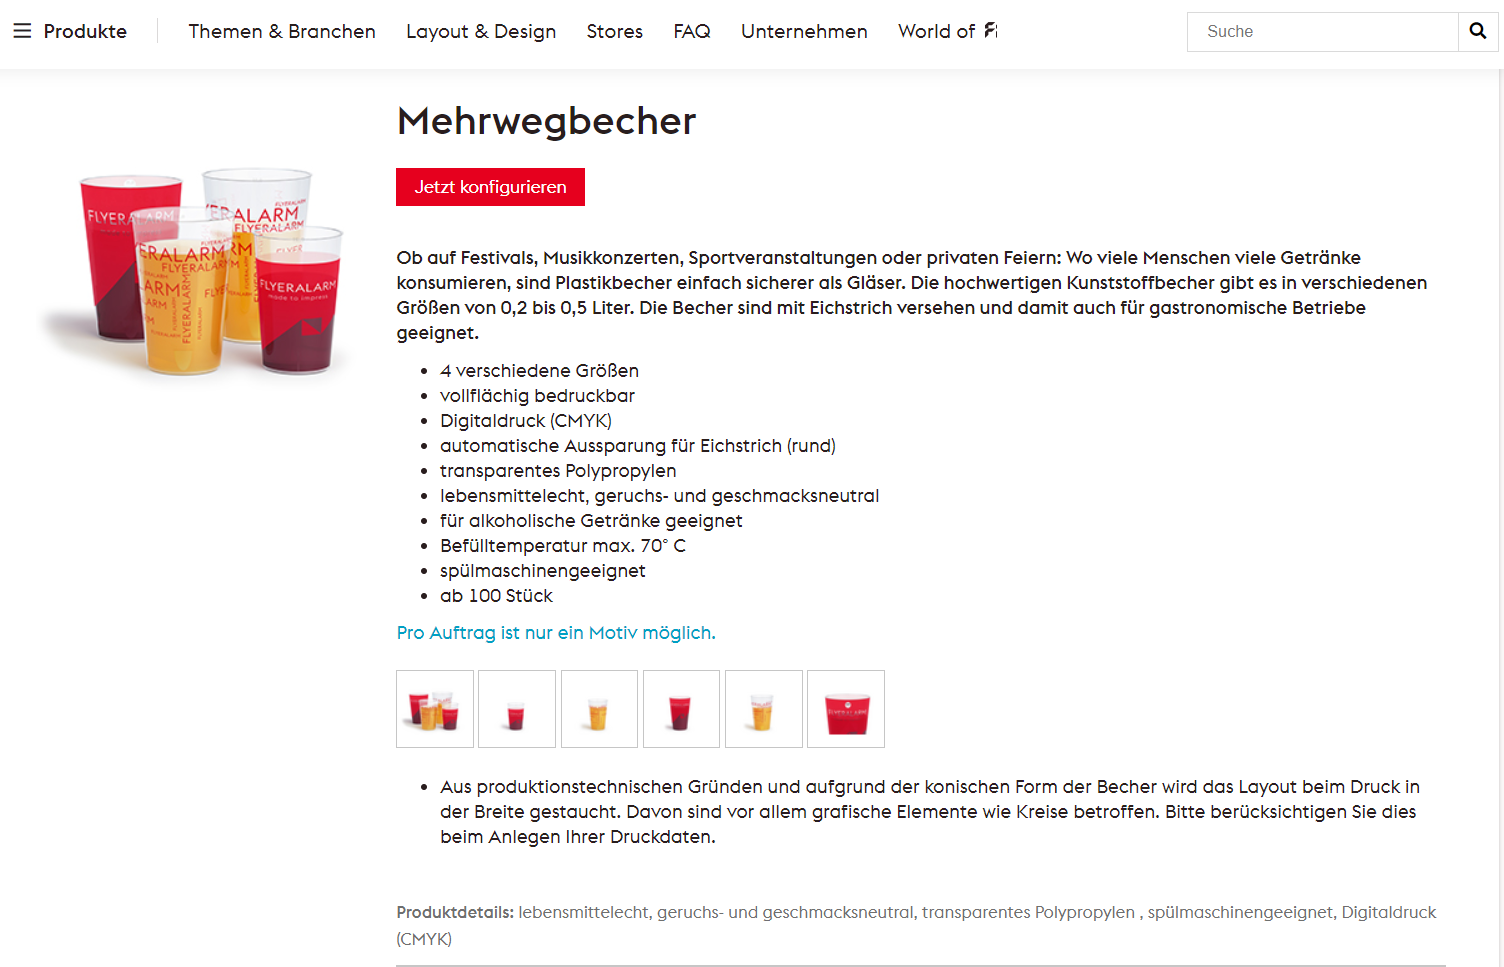
\epsfig{file = technik/images/flyeralarm.png, width=11.0cm}}
	\caption[Mehrwegbecher bestellen]{\textit{Bestellvorgang von Mehrwegbechern auf flyeralarm.com}}
	\label{fig:flyeralarm}
\end{figure}
% 
Dazu muss man, nachdem man die gewünschte Größe gewählt hat, sein Design hochladen. Dabei sollte man das Datenblatt\footnote{Das Datenblatt ist auf der Webseite zu finden und kann von dort heruntergeladen werden.} berücksichtigen, welches die Vorgaben beschreibt wie zum Beispiel Sicherheitsabstand oder Druck Farbraum. Die Online-Druckerei schreibt auf ihrer Webseite:\textit{\glqq Aus produktionstechnischen Gründen und aufgrund der konischen Form der Becher wird das Layout beim Druck in der Breite gestaucht. Davon sind vor allem grafische Elemente wie Kreise betroffen.\grqq} \cite{flyeralarm_mehrwegbecher_nodate} Eine Vorschau, wie das ganze am Ende aussehen wird, gibt es nicht. Im schlechtesten Fall hat man am Ende ein nicht zufriedenstellendes Ergebnis. Auch andere Seiten bieten ein ähnliches Angebot.Eine fertige Vorschau ist jedoch eher nicht zu finden.
%
\subsection{Spread Shirt}
\label{sec:spreadshirt}
%
Spreadshirt ist eigentlich eine Onlinedruckerei für T-Shirts. Sie selbst schreiben über sich Folgendes: \textit{\glqq Seit 2002 liefert Dir Spreadshirt T-Shirt-Druck in bester Qualität. Was als Start-up-Idee in Leipzig begann, ist inzwischen ein weltweit erfolgreiches Print-on-Demand-Unternehmen, das Wert auf faire Handels- und Produktionswege legt, seine Verantwortung als internationaler Arbeitgeber ernst nimmt und seinen Mitarbeitern ein attraktives Arbeitsumfeld bietet.\grqq } \cite{spreadshirt_tassen_nodate}
%
\begin{figure}[h]
	\centering
	{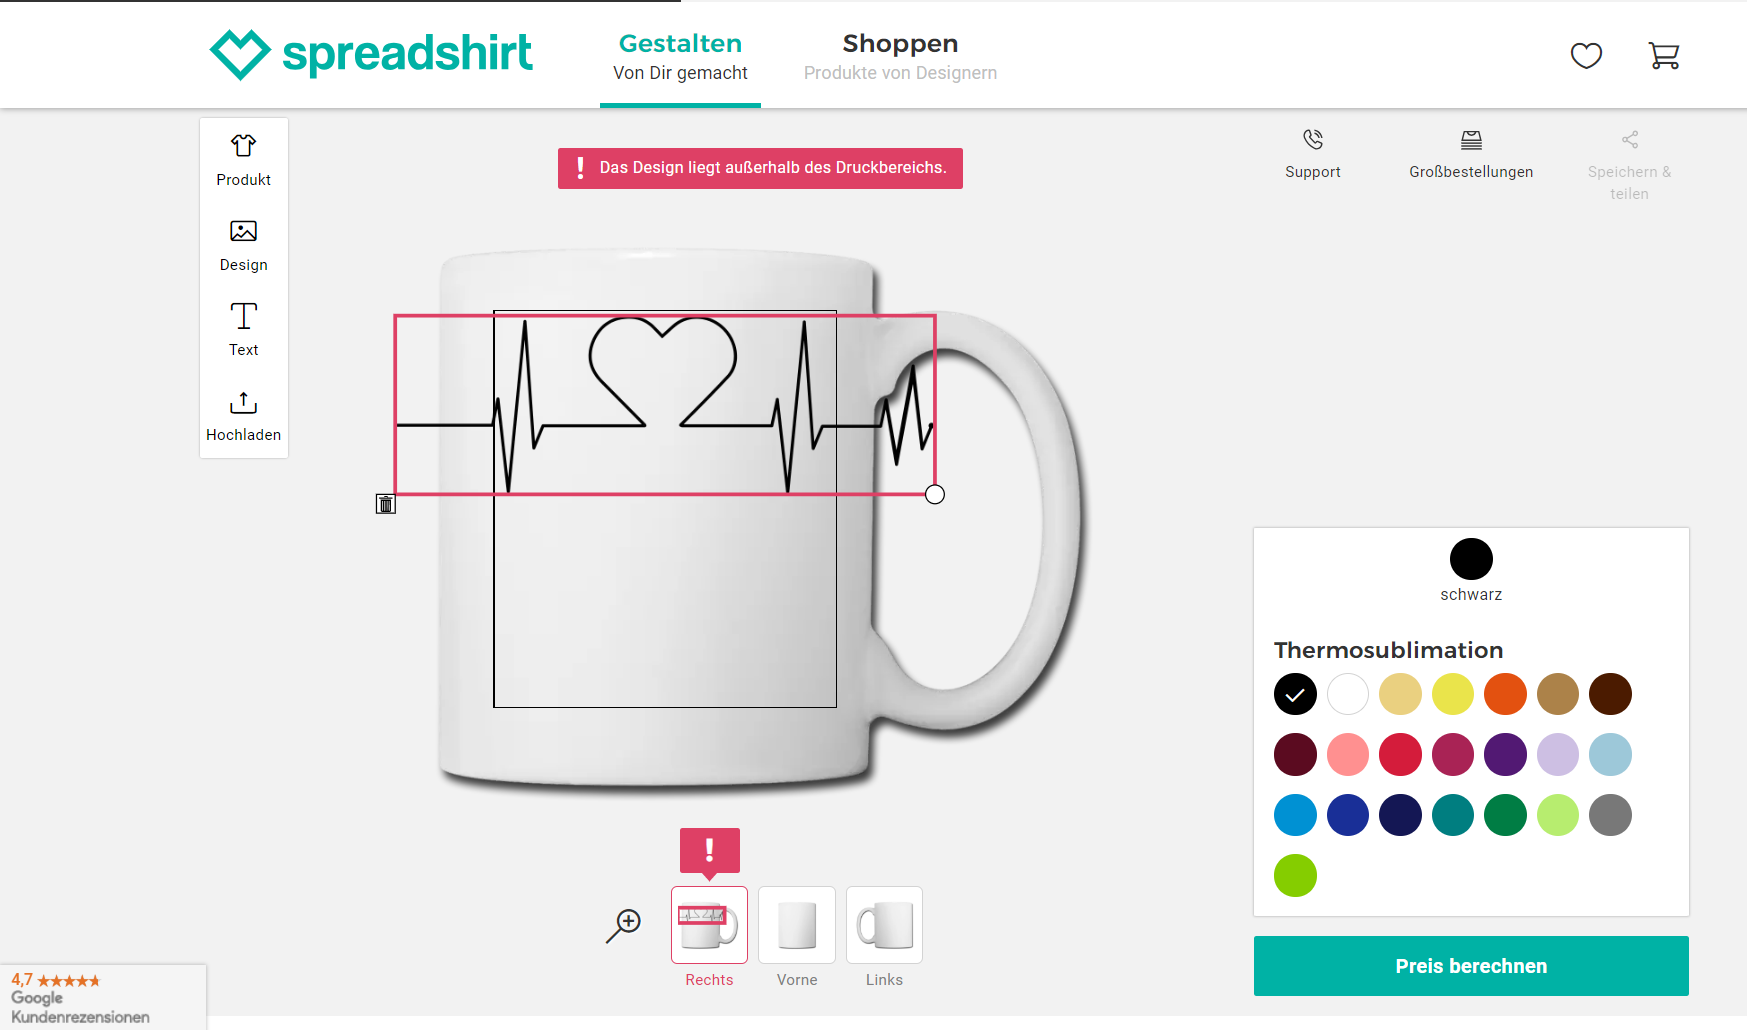
\epsfig{file = technik/images/spread-shirt.png, width=11.0cm}}
	\caption[Tasse bestellen]{\textit{Gestaltung einer Tasse auf spread-shirt.com}}
	\label{fig:spread}
\end{figure}
%
Zwar wird kein Druck von Mehrwegbechern angeboten, dafür aber der Druck von Tassen. Der Kunder kann hier in einem Online-Konfigurator seine Tasse selbst gestalten, indem er Text oder Bildelemente auf die Tasse legt. Das ganze wird sogar in 3D angezeigt. Jedoch ist die Ansicht nicht flexibel sondern statisch. Man kann die Tasse lediglich von drei verschiedenen Blickwinkeln betrachten (rechts, vorne, links). In unserem Fall sollen fertige Designs dargestellt werden. Auch das ist beim Tassenkonfigurator von Spreadshirt schwierig. Wie in der Abbildung \ref{fig:spread} zu sehen kann ein Objekt nur im Druckbereich dargestellt werden, nicht außerhalb des Bereichs. Damit ist ein Rundum-Druck nicht möglich. \\
Trotzdem lässt sich sagen, dass dieser Konfigurator gut und übersichtlich gestaltet ist. Jedoch hat er nicht die Funktionalität, welche der Konfigurator für Gizeh haben sollte.
%
\subsection{Becher-bedrucken.de}
\label{sec:currycup}
%
Ein weiteres Angebot für Becher gibt es auf \textit{becher-bedrucken.de}. Dort gibt es einen 3D Konfigurator für verschiedene Becher. Der technische Ansatz ist schon sehr gut und kann bei der Entwicklung berücksichtigt werden. Es werden ähnliche Technologien verwendet, wie in dieser Arbeit. Jedoch sind die Designvorgaben ganz anders als die Druckvorgaben von Gizeh. Das hochgeladene Design ist so angepasst, das es bestmöglich auf dem Becher angezeigt werden kann.
%
\begin{figure}[h]
	\centering
	{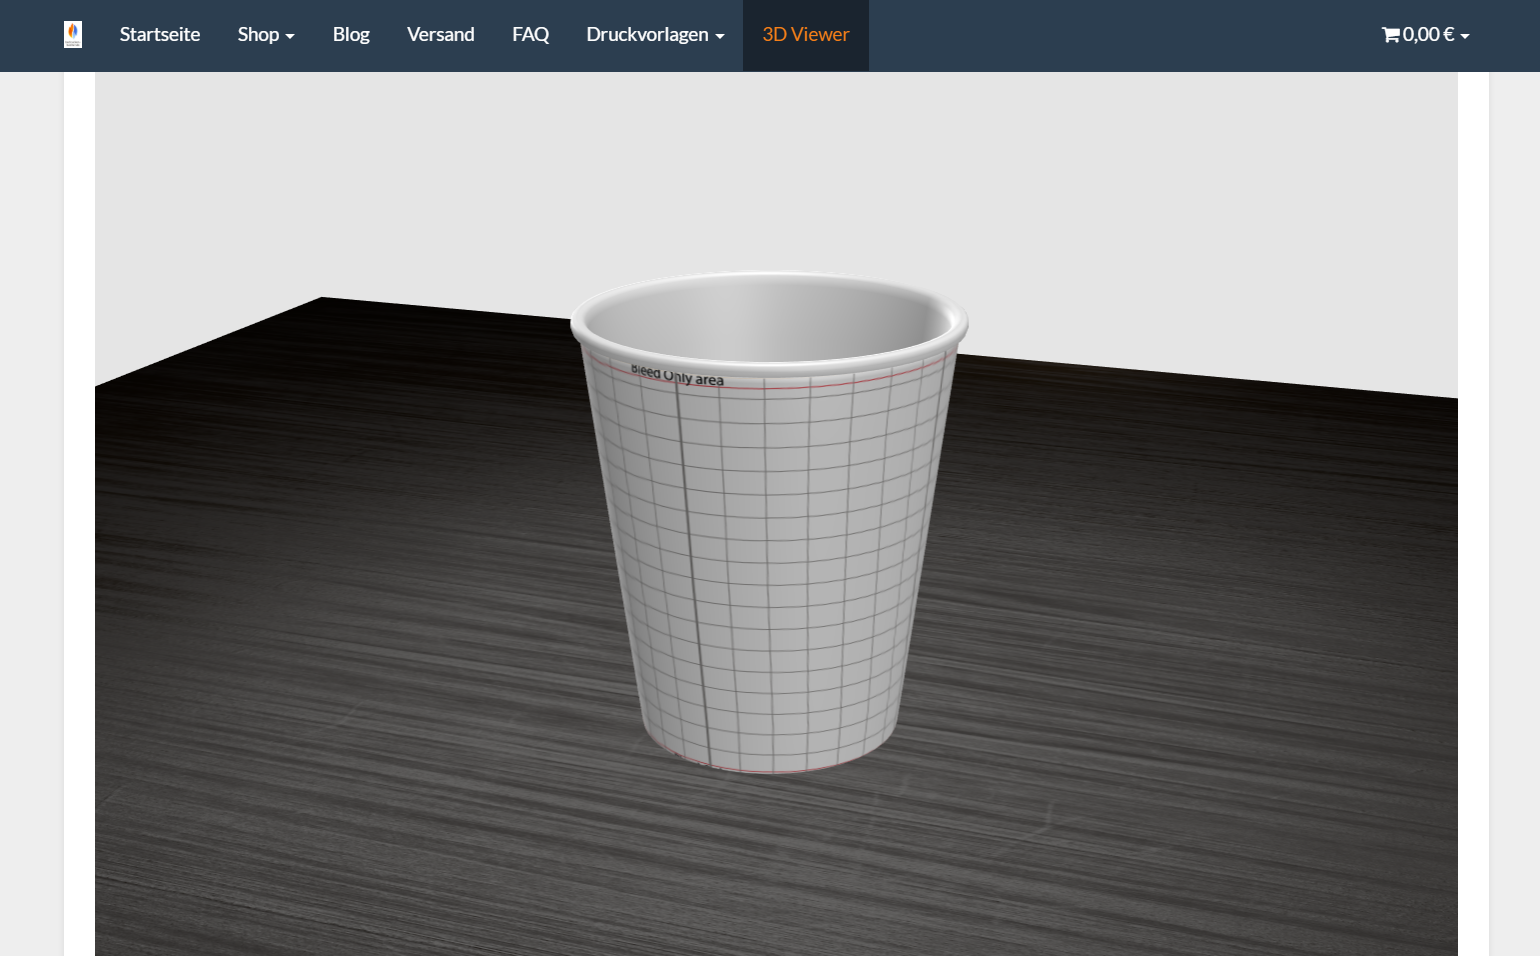
\epsfig{file = technik/images/becher-bedrucken.png, width=11.0cm}}
	\caption[Becher bedrucken]{\textit{3D Viewer eines Bechers auf bedrucken-becher.de}}
	\label{fig:becherbedrucken}
\end{figure}
%
Die Darstellung in 3D ist schön anzusehen. Zumindest auf einem Gerät mit größerem Display. Eine Anpassung für mobile Geräte ist so gut wie gar nicht vorhanden. Technisch gesehen kann aber trotzdem an diesen Lösungsansatz angeknüpft werden.
%
\section{3D Online Konfiguratoren}
\label{sec:3dconfigurators}
%
Heutzutage kann nahezu alles bedruckt werden. Die Vielzahl an Produkten ist groß. Dies haben wir bisher in diesem Kapitel erläutert, wie das konkret bei Bechern oder Tassen aussehen kann. Schwieriger zu finden sind allerdings 3D Konfiguratoren für diese Produkte. Oft gibt es höchsten eine 3D Pop-Up Ansicht, eine alte Lösung mit Flash o. ä. Eine responsive Lösung ist eher nicht zu finden. \\
In der Autoindustrie und anderen Branchen sind jedoch einige gute 3D Konfiguratoren umgesetzt. Wenn man eventuell die passenden Felgen sucht, bekommt man da einen übersichtlich gut gestalteten Konfigurator in 3D. Teilweise sind Konfiguratoren zu finden, welche responsiv sind. Einige Firmen bieten sogar an 3D Konfiguratoren für bestimmte Produkte umzusetzen. Dabei handelt es sich meist um individuelle Lösungen. Das Folgende Beispiel soll zeigen, das es durchaus möglich ist gute 3D Konfiguratoren zu entwickeln.
%
\begin{figure}[]
	\centering
	{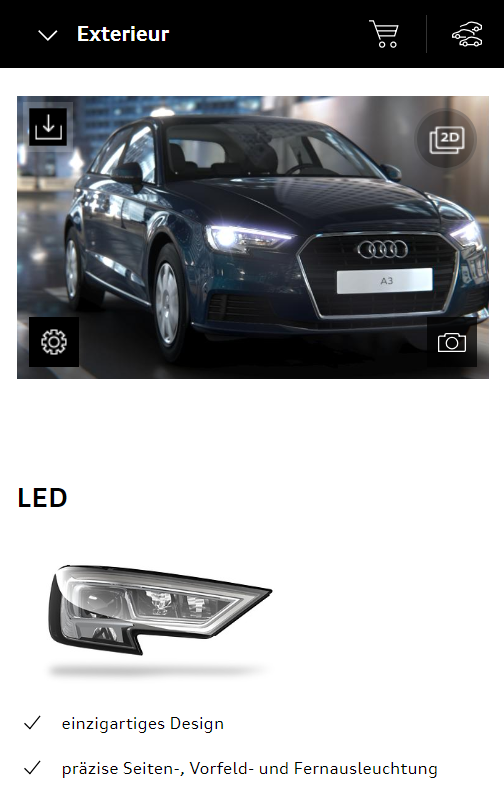
\epsfig{file = technik/images/audi.png, width=6.0cm}}
	\caption[Audi Konfigurator]{\textit{Neue 3D Ansicht von Audi}}
	\label{fig:audi}
\end{figure}
%
%
\paragraph{Audi 3D Konfigurator}Letztes Jahr veröffentlichte Audi seinen neuen Konfigurator auf der Webseite. Er rendert die Fahrzeuge in Echtzeit. Die Anwendung ist auch für mobile Geräte optimiert (siehe Abbildung \ref{fig:audi}). So kann man den Konfigurator beispielsweise mit Toucheingaben steuern. Man kann sich das Fahrzeug ganz genau anschauen und an Details heranzoomen. Technisch eine sehr gute Umsetzung, die auch optisch etwas her macht. \\
%
Bei dem 3D Konfigurator für Mehrwegbecher soll zusätzlich ein eigenes Design gerendert werden. Eine wirklich zufriedenstellende Lösung gibt es da nicht. Mit aktuellen Technologien, könnte ein Lösung umgesetzt werden. Diese sind oft noch sehr jung und wenig dokumentiert, aber haben gute Voraussetzungen um eine Lösung zu entwickeln.
%
\section{Webframeworks}
\label{sec:webframeworks}
%
Wofür es früher Flash gab, werden nun Frameworks wie \textit{Angular} oder \textit{ReactJS} verwendet. Es handelt sich dabei um Frontend Frameworks für Webapplikationen. Dabei hat man heutzutage oft die Qual der Wahl. Die Anzahl der Angebote an Frameworks und Libraries ist groß. Sie kommen oft beim Entwickeln von \textit{Single Page Applications (SPA)}  zum Einsatz.
%
\paragraph{Angular}
\label{p:angular}
%
ist nichts anderes als ein JavaScript-Framework auf Basis von TypeScript\footnote{Eine von Microsoft entwickelte Programmiersprache. TypeScript ist eine kompilierte und plattformübergreifende Sprache, die reine JavaScript-Dateien generiert.}. Es wurde von Google entwickelt und ist ein Open-Source-Framework. Es unterstützt den Entwickler dabei, moderne Webanwendungen zu machen, die zum einen für Desktop und zum andern für Mobile optimiert worden sind. Wie in der Abbildung \ref{fig:googletrends} zu sehen, ist \textit{Angular} das meist genutzte und bekannteste Framework für SPAs. Ähnliches zeigt auch die Stack Overflow Entwicklerumfrage 2018: Bei den meist genutzen Bibliotheken und Frameworks liegt Angular mit 36,9\% einen Platz vor React mit 27,8\% \cite{stackoverflow_stack_2018}.
%
\begin{figure}[h]
	\centering
	{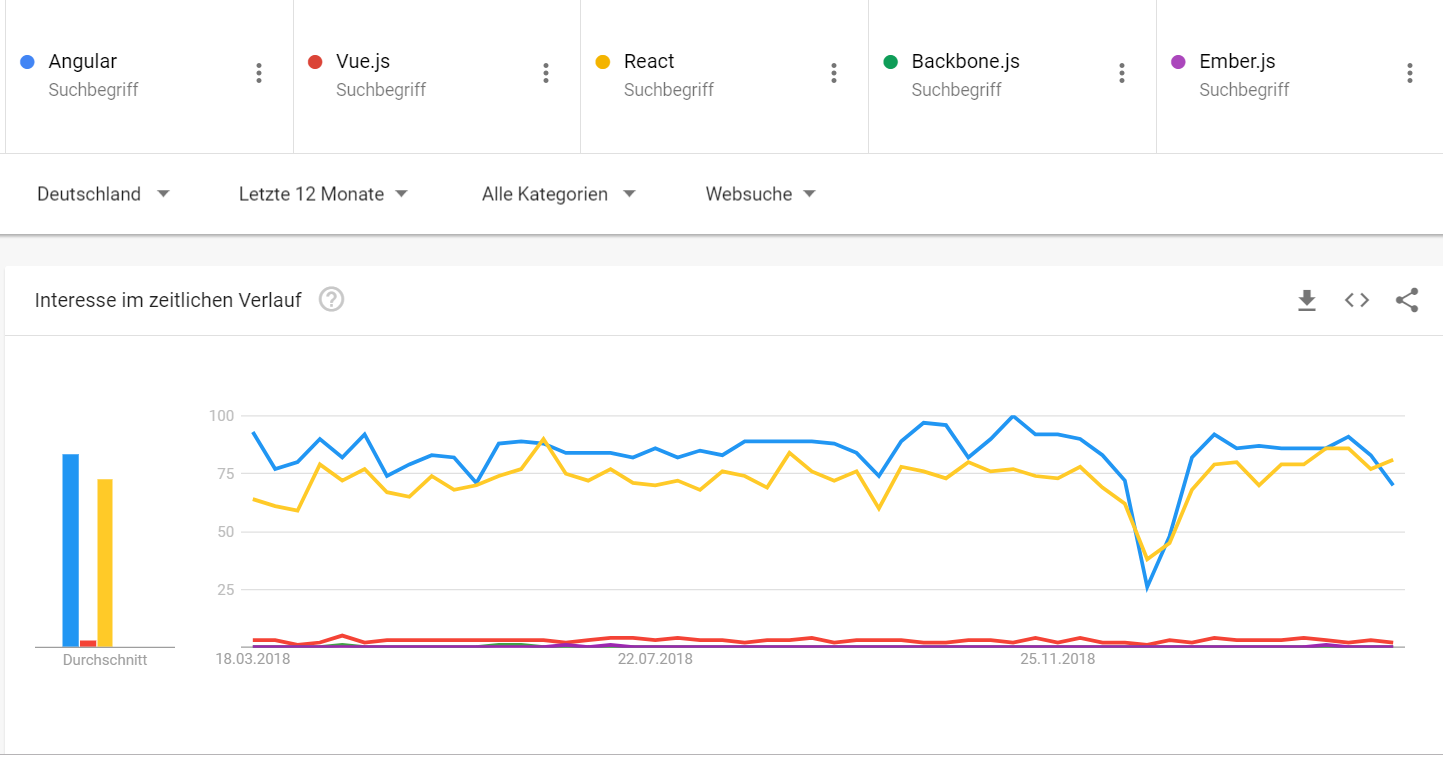
\epsfig{file = technik/images/google-trends.png, width=13.0cm}}
	\caption[Audi Konfigurator]{\textit{Google Trends Statistik. Suchanfragen von Frontend-Frameworks in 2018}}
	\label{fig:googletrends}
\end{figure}
%
Außerdem gibt es den Entwicklern Konventionen und Richtlinen an die Hand. Das ist gerade dann sinnvoll, wenn man in einem großen Team arbeitet. Oder bei großen Projekten für ein einfaches Handling und die Wartbarkeit des Codes sinnvoll wird. Ein Merkmal von Angular ist, das es viele unterschiedliche Module gibt, die es ermöglichen, sehr effizient Anwendungen zu produzieren. Da gibt es Module, welche für die Client-Server-Kommunikation zuständig sind. Sie ermöglichen die Kommunikation mit dem Backend. Ein anderes Modul ist für die Bindung der Daten zuständig. Wenn ich auf einer Ansicht Informationen bereitstellen möchte, die zum Beispiel aus einer Datenbank kommen, kann ich das ganz einfach mit dem Bindungsmechanismus von Angular umsetzen. Das Framework ist auch bekannt für seine tollen Animationen auf Basis von Web-Animation. Ein weiteres, wichtiges Modul ist das Routing-Modul. Im Grunde genommen sind Routings Grundbestandteil für \textit{Single Page Anwendungen}. Mittels Routings kann ich festlegen welcher Teil der Anwendung nun angezeigt werden soll. Außerdem baut das Framework auf die komponentenbasierte Programmierung. In Kapitel 3 werden wir noch genauer auf Angular eingehen\footnote{Die Dokumentation des Frameworks ist unter \textit{https:/angular.io/docs/} zu finden.}.
%

%
\paragraph{React}
\label{p:react}
%
ist das meistgesuchte JavaScript Framework 2018 \cite{stackoverflow_stack_2018}. Es wurde 2013 von Facebook entwickelt und viele bekannte Unternehmen wie Netflix, Twitter oder PayPal verwenden das Framework. Ähnlich wie Angular setzt React auf modulare Komponentenarchitektur. Damit wird der Frontendcode leicht nachvollziehbar. \textit{\glqq Das Ziel von React ist es, einfacheren Code schreiben zu können, dessen Bestandteile weniger miteinander verschränkt oder verwoben sind \grqq}\cite{kogel_paul_react_2015} \\
React ist kein Framework, es ist eine Bibliothek. Es ist ein sehr flexibles Werkzeug, dass in bestehende Anwendungen eingebaut werden kann, ohne den ganzen Code umzustrukturieren. Dem Entwickler wird keine Grundstruktur für seine Applikation gegeben, was ein wesentlicher Unterschied zu Angular ist. Ein weiteres Merkmal von React ist die virtuelle DOM. Diese garantiert die Synchronisierung der DOM indem bei Änderungen alles neu gerendert wird\footnote{Die vollständige Dokumentation ist unter \textit{https://reactjs.org/docs/getting-started.html} zu finden}.
%
\paragraph{Vue.js}
\label{p:vueJS}
%
ist ein weiteres Frontend-Framework zur Entwicklung von \textit{Single Page Anwendungen}. Es ist nicht das beliebteste Framework und trotzdem taucht es immer wieder auf (siehe Abbildung \ref{fig:googletrends}) und ist definitiv eine Alternative zu \textit{Angular} oder \textit{React}. Es setzt auch auf eine modulare Architektur, die in einzelne Komponenten zerteilt ist. Das Framework ist im Vergleich zu seinen Konkurrenten deutlich einfacher und hat eine flache Lernkurve. Dadurch ist es auch schneller und bringt dem Framework einen Vorteil gegenüber den Alternativen. Obwohl es kleiner ist, bringt es trotzdem alle wichtigen Funktionen wie Suchmaschinenoptimierung mit sich. Es kann auch in Kombination mit React verwendet werden. In Vue.js wird ohnehin das bekannte virtul DOM genutzt. Auch die Community ist stetig am wachsen.\footnote{Weitere Informationen sind in der offizielen Dokumentation unter \emph{https://vue.js.org/v2/guide} zu finden.} \\
%
%
%
%%%%%%%%%%%%%%%%%%%%%%%%%%%%%%%%%%%%%%%%%%%%%%%%%%%
%
% A U F B A U 
%
%%%%%%%%%%%%%%%%%%%%%%%%%%%%%%%%%%%%%%%%%%%%%%%%%%%
%
\section{Flash und WebGL}
\label{sec:webgl2}
%
In dem Artikel \emph{HTML5/WebGL vs Flash in 3D Visualisation} schreibt der Autor folgendes über WebGL:\\

\textit{\glqq Die Entwicklung verbesserter 3D-Grafiken in webbasierten Anwendungen hat in letzter Zeit einen Schritt vorwärts getan, als Programmierer WebGL in die Mozilla Firefox Nightly-Builds und in WebKit integriert haben, das in Google Chrome und dem Safari-Browser von Apple verwendet wird. WebGL ist eine der am meisten entwickelten Bibliotheken, die von HTML5 unterstützt werden.\grqq } \cite{bahor_html5/webgl_2013}.\\

Adobe Flash ist auch heute noch vielen ein Begriff. Es war darauf ausgerichtet interaktive 2D Grafiken im Web bereitzustellen. Mit der Veröffentlichung der Version 10 des Flash Players haben die Entwickler sogar eine z-Achse eingeführt. Sie ermöglicht eine 3D Darstellung und Transformation von Objekten. Diese Unterstützung für die Interaktion von Objekten der dritten Dimension wurde jedoch in begrenzter Weise bereitgestellt.\\
Einer der aktuellsten Leistungstests zwischen dem Flash- und dem WebGL-Canvas-basierten 3D-Inhalt zeigt deutlich, dass der HTML5-Canvas beginnt, höhere Frameraten zu generieren und 3D-Inhalte im Web zu rendern. Die Testergebnisse zeigen, dass WebGL beim Rendern von 3D-Inhalten wesentlich schneller abschneidet und höhere Frameraten für die 3D-Animationen im Web bietet, während sie mit Flash verglichen werden. Weiter schreibt Senad Bahor in seinem Artikel, dass \textit{es eigentlich bei der 3D-Grafik darum geht, dass 3D-Modell zu ändern und zeitabhängig zu sehen. Dies kann derzeit nur durch die Verwendung der HTML5- und WebGL-Engines im Web erreicht werden, da HTML5 Interoperabilität zwischen verschiedenen Elementen (sowohl traditionellen als auch HTML5-basierten) bietet, während JavaScript dazu veranlasst wird, die Renderprozedur durch den WebGL-Prozess zu handhaben.}\cite{bahor_html5/webgl_2013}\\
Weiter zeigen die Ergebnisse des Artikels deutlich, dass Flash-basierte 3D-Grafiken auf iOS-basierten Geräten nahezu nicht darstellbar sind, da Adobe mit seinem Flash-Plugin nie iOS unterstützt hat. Aufgrund der HTML5-Funktionalität und -Erreichbarkeit kann die Webseite auch auf einer Vielzahl von Geräten, einschließlich iOS- und Android-Geräten, wiedergegeben werden, ohne dass sich die Benutzer um das Vorhandensein der Plugins und die Versionierung des Players kümmern müssen.
Webbrowser entwickeln sich stetig weiter. WebGL kann in über 95\% aller Browser verwendet werden \cite{deveria_alexis_can_2013}. Was zuvor schon in Videopielen mit OpenGL möglich war, ist nun auch im Web möglich. Wie genau WebGL als Abstraktionsschicht für den grafischen Teil einer Anwendung verwendet werden kann, wird in Kapitel \ref{sec:javascriptbibliotheken} erläutert.

Mit WebGL müssen die Benutzer nicht dazu aufgefordert werden, eines der Plugins zu installieren, um den 3D-Inhalt auf der Website zum Laufen zu bringen. Die einzige Voraussetzung ist, dass der Webbrowser das HTML5-Canvas-Element unterstützt, über das WebGL den Inhalt für den Benutzer darstellt.\\
Im Wesentlichen kann WebGL auf jeder Plattform und auf allen großen Systemen mit OpenGL-fähiger Grafikkarte und einem Browser ausgeführt werden, der WebGL unterstützt.\\

\section{3D JavaScript Bibliotheken}
\label{sec:javascriptbibliotheken}
%
Um eine 3D Szene mit WebGL darzustellen wird ein JavaScript Framework benötigt. Es erstellt und rendert eine Szene mit den 3D Objekten. Im Folgenden werden die zwei bekanntesten und weit verbreitetsten Bibliotheken vorgestellt.
\paragraph{ThreeJS}
\label{sec:threeJS}
%
\textit{Three.js} ist es eine sehr seriöse WebGL-Bibliothek mit einer starken Community und vielen guten Beispielen. Es wird auch oft in kommerziellen Webanwendungen verwendet. Die erste Version des Frameworks tauchte 2010 auf und der Quellcode wird in einem Repository auf GitHub gehostet\footnote{https://github.com/mrdoob/three.js/}. Three.js hat eine verständliche Struktur und große Anpassungsmöglichkeiten. Es ist eine Anwendungsprogrammierschnittstelle, mit der animierte 3D-Grafiken in einem Webbrowser erstellt und angezeigt werden. Neben der Dokumentation gibt es auch ein Wiki, was dem Entwickler zum schnellen Einstieg sehr helfen kann\footnote{https://github.com/mrdoob/Three.js/wiki/}.Schon beim erstellen einer einfachen Szene mit dem Framework fällt auf, das es dem Prinzip der objektorientierten Programmierung folgt\footnote{https://threejs.org/docs/\#manual/en/introduction/Creating-a-scene}. In dem Kapitel \ref{cha:introduction} wird noch genauer auf das Framework eingegangen.
%
%\begin{figure}[h]
%	\centering
%	{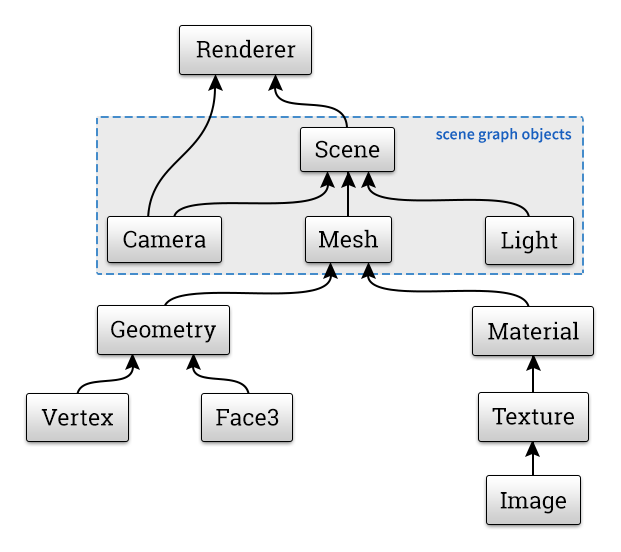
\epsfig{file = technik/images/node-map.png, width=11.0cm}}
%	\caption[Audi Konfigurator]{\textit{Aufbau einer Szene in Three.js}}
%	\label{fig:threejs}
%\end{figure}
%
%
\paragraph{BabylonJS}
\label{sec:babylonJS}
%
Babylon.js\footnote{Die offizielle Dokumentation ist unter \textit{https://doc.babylonjs.com/} zu finden.} ist ein Framework, mit dem komplette 3D-Webanwendungen erstellen werden können. Babylon.js hat eine Community, die stetig wächst und auch aktiv zum Projekt beiträgt und immer mehr Funktionen hinzufügt. Das Framework hat alle notwendigen Werkzeuge, um 3D-Anwendungen umzusetzen. Sie können 3D-Objekte laden und zeichnen, diese 3D-Objekte verwalten, Spezialeffekte erstellen und verwalten, räumliche Sounds spielen und verwalten, Gameplay erstellen und vieles mehr. 
%
\begin{figure}[h]
	\centering
	{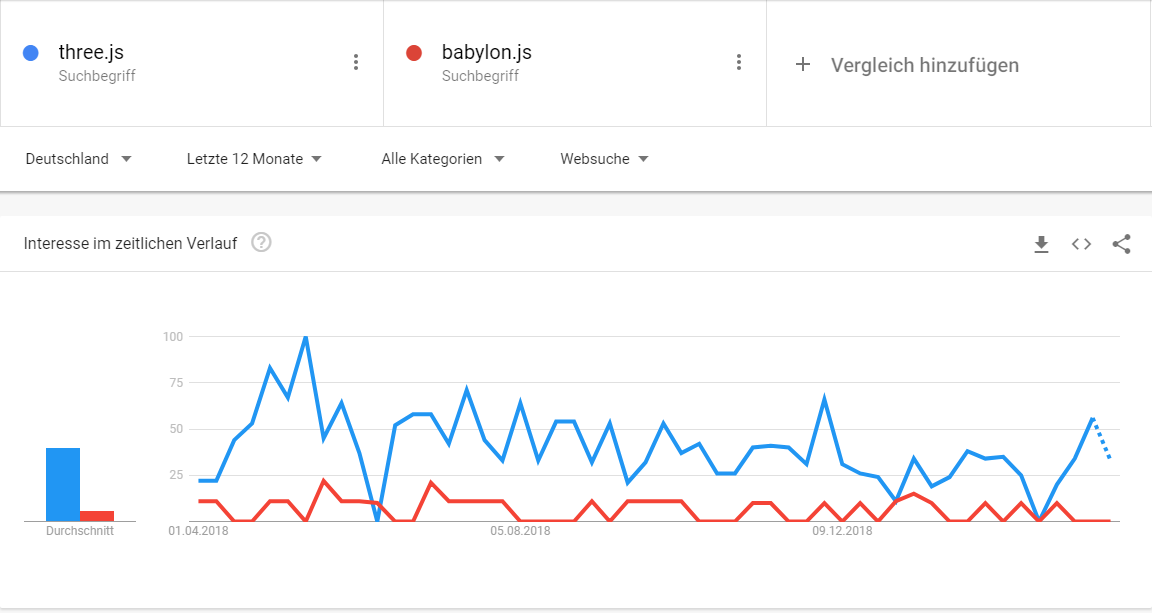
\epsfig{file = technik/images/3d-framework.png, width=13.0cm}}
	\caption[Audi Konfigurator]{\textit{Google Trends: Vergleich Three.js und Babylon.js in den letzten 12 Montaten}}
	\label{fig:compare3dframework}
\end{figure}
%
Babylons.js ist ein benutzerfreundliches Framework, da Sie diese Dinge mit den minimalen Codezeilen einrichten können. Es ist ein mit TypeScript entwickeltes JavaScript-Framework. \cite{moreau-mathis_babylon.js_2016} Wie in Abbildung \ref{fig:compare3dframework} zu sehen ist Babylon.js jedoch weniger gefragt als three.js. Das zeigt sich auch in den 3D Webanwendungen, wo auch meist three.js verwendet wird.

		
		%---- Kapitel Grundlagen ----
		%
%%%%%%%%%%%%%%%%%%%%%%%%%%%%%%%%%%%%%%%%%%%%%%%%%%%
%
%  E N T W I C K L U N G S U M G E B U N G
%
%%%%%%%%%%%%%%%%%%%%%%%%%%%%%%%%%%%%%%%%%%%%%%%%%%%
\chapter{Grundlagen}
\label{cha:grundlagen}
%
%
In dem Grundlagenkapitel geht es um das Basiswissen, auf dem die Arbeit aufbaut. Es wird näher auf die verwendeten Technologien eingegangen. Dabei werden die Frontend-Frameworks beleuchtet sowie die 3D Bibliotheken. Näher wir auch auf die Begriffe Resposive Webdesign, Usability und Performance eingegangen.
%
%
%%%%%%%%%%%%%%%%%%%%%%%%%%%%%%%%%%%%%%%%%%%%%%%%%%%
%
% S P A
%
%%%%%%%%%%%%%%%%%%%%%%%%%%%%%%%%%%%%%%%%%%%%%%%%%%%
%
\section{Single Page Anwendungen}
\label{sec:spa}
%
Früher war es bei Webanwendungen wichtig, soviel wie möglich auf dem Server zu erledigen. Bei modernen Webframeworks gilt jedoch genau das Gegenteil. Es wird versucht möglichst viel clientseitig umzusetzten.\textit{\glqq Dies steigert die Benutzerfreundlichkeit und schafft die Möglichkeit der Anpassung an die Auflösungen und Formfaktoren der vielen unterschiedlichen klassischen und mobilen Plattformen.\grqq } \cite{bahor_html5/webgl_2013}. Im Folgenden wird nun kurz etwas genauer darauf eingegangen was André Krämer in seinem Videokurs sehr gut und einfach erklärt hat.
%
\paragraph{Klassische Webanwendungen}
%
Bevor man sich damit befasst was Single Page Anwendungen sind, sollte man sich das Prinzip einer klassischen Webanwendung anschauen. Nehmen wir beispielsweise an, ein Client sendet eine Anfrage an einen Server. Hierbei handelt es sich um einen Webbrowser, welcher eine Webadresse öffnen möchte. Der Zielserver übernimmt die Verarbeitung. In der Regel laufen nun Skripte auf dem Server, welche HTML rendern. Schließlich bekommt der Client auf seine Anfrage eine Antwort in Form eines HTML-Dokumentes und kann es dann anzeigen. Bei diesem Vorgang liegt die komplette Verarbeitung bei dem Server. Der Webbrowser dient lediglich der Darstellung und einfachen Eingabe. Das die Daten auf einem Server verarbeitet werden wird deutlich, wenn ein Seitenwechsel vorgenommen wird. Dabei wird kurze Zeit nichts angezeigt während die Seite komplett neu lädt.\\
Mit der Einführung von AJAX\footnote{Ajax bzw. AJAX steht als Akronym für „Asynchronous JavaScript and XML“. Die Technologie ermöglicht es, einzelne Teile einer Webseite bei Bedarf asynchron zu laden, so dass sie dynamisch wird. Der angezeigte Inhalt lässt sich gezielt so manipulieren, ohne die komplette Seite neu zu laden.} in 2005 machte die Webentwicklung einen Schritt nach vorne. Nun war es nämlich möglich, Daten asynchron an den Server zu senden. Das heißt, der Server verabreitet zwar immer noch die Daten, sendet nun aber nur noch einen Teil des vorgerenderten Dokuments oder sogar nur einzelne Daten der Seite. Somit wird die Seite nicht wieder komplett neu geladen. Wenn man nun aber in einen komplett andern Bereich der Seite wechseln will, hilft AJAX nicht. Die Seite wird neu geladen und es dauert einen kurzen Moment bis das Ergebnis vom Webbrowser angezeigt werden kann. Um dieses Problem zu lösen, kommen \textit{Single Page Anwendungen} zum Einsatz.
\paragraph{Dezentralisierung der Webanwendung}
%
Im Grunde arbeiten SPA's nach folgendem Prinzip: Der Webbrowser sendet eine Anfrage an den Server. Dieser verarbeitet, wie bei klassischen Webanwendungen nun die Anfrage. Anschließend wird im Webbrowser eine Benutzeroberfläche dargestellt. Nun kommt der entscheidende Unterschied zu klassischen Anwendungen. Bei einem Seitenwechsel oder anderen Interaktionen des Benutzers wird eine neue Benutzeroberfläche erzeugt, indem Teile der Seite ausgetauscht werden. Die Seite wird nie komplett neu geladen. Der Nutzer bleibt immer auf der einen Seite, zumindest fühlt es sich für den Benutzer so an. Dieses Prinzip kennt der Anwender von Desktop-Anwendungen. Man hat sogar die Möglichkeit die Anwendung (zumindest teilweise) offlinefähig zu machen.\\
Die Grundlage einer solchen Anwendung ist das Routing. Abhängig vom Pfad werden bestimmte Bausteine der Anwendung angezeigt bzw. ausgeblendet. Wie wir im späteren Verlauf dieser Arbeit noch sehen werden, hat man tatsächlich nur eine HTML-Datei, welche abhängig vom Kontext immer andere Inhalte anzeigen kann.\\
%
Zusammenfassend lässt sich also festhalten, das ein Ziel von SPAs ist, die Kommunikation zwischen Client und Server enorm zu reduzieren. Um dies zu erreichen wird die Anwendung dezentralisiert. Das heißt, es gibt nur ein HTML Dokument\cite{domin_was_2018}. Durch den Einsatz von Frameworks, wie Angular, ist es möglich Inhalte zu aktualisieren oder zu einer anderen Seite zu wechseln, ohne die Seite über den Server neu zu laden.
\footnote{Das Prinzip von Single Page Anwendungen wird zum Beispiel von Googles Gmail und Gmaps sowie von Twitter verwendet}
%
%
%%%%%%%%%%%%%%%%%%%%%%%%%%%%%%%%%%%%%%%%%%%%%%%%%%%
%
% A U F B A U 
%
%%%%%%%%%%%%%%%%%%%%%%%%%%%%%%%%%%%%%%%%%%%%%%%%%%%
%
\section{Framework Angular}
\label{sec:angular7}
Das Framework Angular ist sehr umfangreich. Im Folgenden werden einige Grundlagen erläutert, die zur Implementierung einer Anwendung mit Angular benötigt werden. Dabei soll ein Grundverständis vermittelt werden, wie das Framework aufgebaut ist und wie es arbeitet.
\subsection{Komponentenbasierte Programmierung}
%
Angular ist ein Framework, das auf Komponenten setzt. Das Prinzip der komponentenbasierten Entwicklung kommt nicht nur bei Angular vor, sondern auch bei vielen anderen Programmiersprachen und Frameworks. Was in Angular Komponenten sind wird in dem Buch \textit{Angular: Grundlagen, fortgeschrittene Techniken und Best Practices mit TypeScript - ab Angular 4, inklusive NativeScript und Redux} folgendermaßen beschrieben:\\
%

\textit{\glqq Komponenten sind die Grundbausteine einer Angular Anwendung. Jede Anwendung ist aus vielen verschiedenen Komponenten zusammengesetzt, die jeweils eine bestimmte Aufgabe erfüllen. Eine Komponente beschreibt somit immer einen kleinen Teil der Anwendung, z. B. eine Seite oder ein einzelnes UI-Element.\grqq }\cite{woiwode_angular:_2017} \\

%
Im Grunde ist eine Komponente also nichts anderes als ein selbstdefinierter HTML-Knoten, den man im HTML Kontext ganz normal nutzen kann. Man erzeugt einfach DOM-Elemente\footnote{Wenn eine Webseite geladen wird, erstellt der Browser eine Document Object Model der Seite. Das HTML-DOM-Modell ist als Baum von Objekten aufgebaut. Diese Objekte sind ein der Regel einfache HTML-Tags} und kann sie dann automatisch in Angular nutzen.
Eine Komponente in Angular ist in drei Parts aufgeteilt: Logik, Vorlage und Style. Die Logik beschreibt die TypeScript Klassen, Eigenschaften, Methoden und so weiter. Sie beschreibt also, was zu tun ist, wenn zum Beispiel ein bestimmter Button geklickt wird. Die Vorlage (Template) ist ein HTML-Schnipsel. Dies kann einfach nur ein Button-Element sein oder auch eine HTML-Struktur mit mehreren HTML-Elementen. Sie beschreibt die Stuktur bzw. den Aufbau der Komponente. Wie die Komponente aussehen soll wird in dem Style Part festgelegt. Dabei ist zu beachten, dass die Style-Definitionen nur innerhalb der Komponente gelten. Globale Styles der Anwendung werden seperat definiert.\\
Der Startpunkt der Anwendung ist die \texttt{index.html}. Sie definiert die Applikationskomponente, der Ankerpunkt einer Angular-Anwendung, quasi eine Basiskomponente. In Dieser können nun weitere Kindskomponenten eingefügt werden, welche auch ineinander verschachtelt sein können. So entsteht eine komplette Struktur. Eine Komponentenvorlage kann also nicht nur HTML-Elemente enthalten, sondern auch Kindskomponenten. Entscheidend ist, das Komponenten verschachtelt werden können. Dies ist das Grundprinzip der komponentenbasierten Programmierung (vgl. Angular Grundkurs\cite{unlu_angular_2018}).

\subsection{Modulare Umsetzung}
Schauen wir uns nun an, wie Angular mit Modulen arbeitet und was genau Module sind. \textit{Nikolas Poniros} hat das in seinem Buch \textit{Angular für Dummies} so definiert:\\

\textit{\glqq Angular-Module helfen beim Gliedern einer Webanwendung in verschiednene Funktionsblöcke. Alle Angular-Bausteine, die logisch zu einem Funktionsblock gehören, werden mit dem entsprechenden Angular-Modul registriert. Die registrierten Bausteine gehören dann zum Angular-Modul. Angular-Module sind von der Denkweise her vergleichbar mit ECMA-Script-Modulen. ECMA-Script-Module kapseln TypeScript-Konstrukte wie Klassen und Funktionen und erlauben nur den Zugriff auf exportierte Konstrukte. Angular-Module kapseln Komponenten, Pipes und Direktiven\footnote{Was genau es mit diesen Angular Bausteinen auf sich hat wird in Punkt \ref{subsec:grundfunktionen} beleuchtet.}. Ein anderes Angular-Modul kann nur auf einen Baustein zugreifen. wenn es dieses exportiert.\grqq \cite{poniros_angular_2019} }\\

Angular bietet also die Möglichkeit modular zu arbeiten. Die einzelnen Elemente und Funktionalitäten können in Modulen gruppiert werden. Im Grunde ist ein Modul nichts anderes als ein Container. Sie lassen sich besonders gut verwenden, wenn man mit mehreren Entwicklern zusammenarbeiten möchte. Module sind einzelne Bestandteile der Anwendung und lassen sich ganz einfach in bestehende Anwendungen einbauen. So kann ich ein Modul in mehreren Anwendungen wiederverwenden. Oder verschiedene Teammitglieder entwickeln jeweils ihre eigenen Module, welche anschließend in einer Anwendung zusammengefügt werden können. Ich kann ein Modul also auch in einem anderen Kontext wiederverwenden. Ein Modul darf allerdings nur in einem einzigen Modul initialisiert werden. Stattdessen wird das Modul bei mehrfacher Verwendung lediglich importiert. Folgendes Beispiel soll das Prinzip modularer Umsetzung verdeutlichen.\\
%
\begin{figure}[h]
	\centering
	{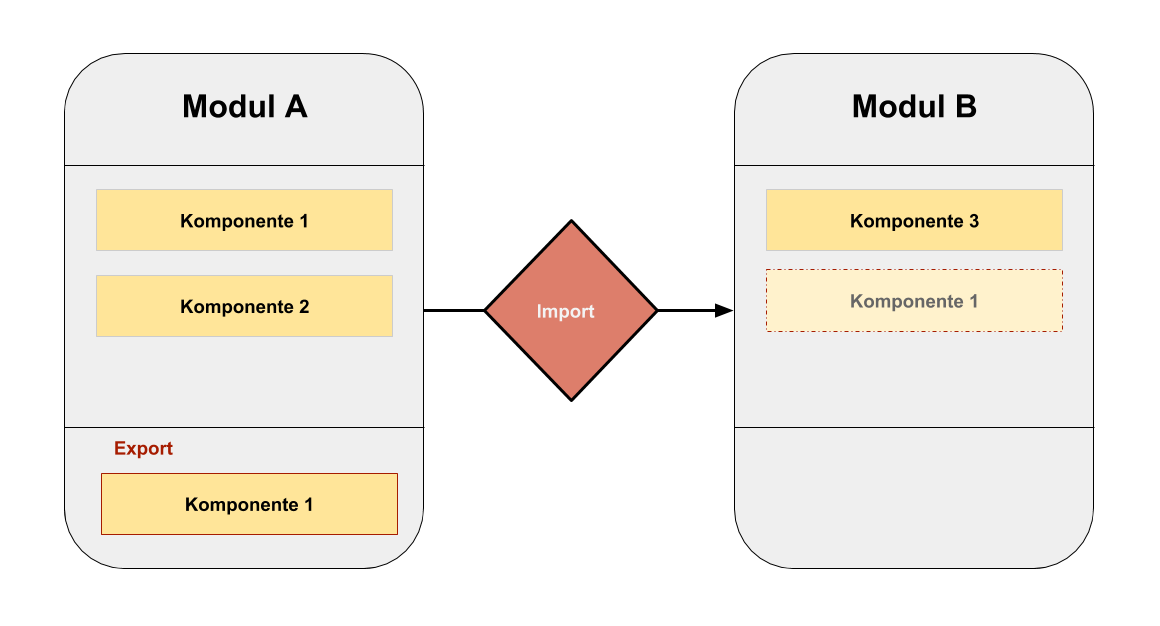
\epsfig{file = grundlagen/images/module.png, width=14.0cm}}
	\caption[Audi Konfigurator]{\textit{Fallbeispiel mit zwei Angular Modulen mit Komponenten}}
	\label{fig:ngModule}
\end{figure} 

%
Das hier beschriebene Beispiel ist in Abbildung \ref{fig:ngModule} zu sehen. Angenommen wir haben ein \textit{Modul A}. In diesem Modul sind nun \textit{Komponente 1} und \textit{Komponente 2} deklariert. Das heißt, es ist möglich in \textit{Komponente 1} die \textit{Kompontente 2} zu verwenden und umgekehrt, weil beide in dem \textit{Modul A} registriert sind. Jetzt haben wir ein weiteres \textit{Modul B}. In diesem ist die \textit{Komponente 3} registriert. Nun wäre es sehr praktisch, wenn \textit{Komponente 3} ebenfalls \textit{Komponente 1} aus dem anderen Modul verwenden könnte. Wie schon erwähnt darf ein Baustein in Angular nur in einem Modul registriert bzw. inititalisiert werden. Deshalb muss das \textit{Modul A} in \textit{Modul B} importiert werden, damit auch dort die \textit{Komponente 1} verwendet werden kann. Zusätzlich muss in \textit{Modul A} die \textit{Komponente 1} exportiert werden. Dadurch wird sie erst von außen frei zugänglich und somit in Bausteinen anderer Module nutzbar.
%
\paragraph{Hauseigene Module}
Angular hat auch ein paar hauseigene Module, die je nach Anwendungsfall importiert werden können. Das \textit{BrowserModule} wird für Web-Anwendungen im Angular-Umfeld genutzt und verfügt über alle Funktionalitäten, mit dem wir in der Lage sind, Ereignisse innerhalb des Browsers abzufangen, DOM-Rendering durchführen zu können und damit schließlich die lauffähige Angular-Anwendung im Browser realisieren zu können.\\
Das \textit{CommonModule} beinhaltet allgemeine Funktionen, die sehr, sehr häufig genutzt werden. Diese Funktionen liegen in Form von Direktiven und Pipes vor, womit ich bestimmen kann, ob ein HTML-Knoten angezeigt wird oder nicht oder auch Pipes, womit ich Ausgaben formatieren kann. Auch sprachabhängige Funktionalitäten sind in den \textit{CommonModule} enhalten.\\
Das \textit{HttpModule} ist dafür da, Client-Server-Kommunikation zu betreiben. Das heißt, HTTP-Requests lassen sich mit Hilfe des \textit{HttpModules} hervorragend realisieren, dafür werden Services zur Verfügung gestellt. Das \textit{HttpModule} hat auch Services für Testings und Co. Für Formulare gibt es entweder das FormsModule oder das \textit{ReactiveFormsModule}. Das hängt so ein wenig davon ab, wie man Formulare in der Anwendung gestalten will.\\
Das \textit{RouterModule} ist dafür da, um Komponenten-Routing zu realisieren. Das Routing ist die Grundlage für \textit{Single-Page-Applications}. Das heißt, über das Routing kann man bestimmen, welche Komponente dargestellt werden muss, wenn ein bestimmter Pfad in der Anwendung besucht wird.
%
\subsection{Grundfunktionen des Frameworks}
\label{subsec:grundfunktionen}
%
Module und Komponenten in Angular haben wir nun schon etwas ausführlicher betrachtet. Nun wollen wir uns weitere Funktionen und Bestandteile von Angular anschauen\footnote{Auf die weiteren Bestandteile von Angular wird hier nicht im Details eingegangen. Genauere Dokumentationen dazu sind online unter angular.io zu finden.}. Wie die einzelnen Bausteine umgesetzt und implementiert werden können sehen wir noch in Kapitel 4 Methodik am Fallbeispiel des 3D Konfigurators für Mehrwegbecher.
%
\paragraph{Bindungen}
%
\textit{\glqq Bindungen sind im Wesentlichen die Brücke zwischen der Darstellungsschicht und der Logikschicht\grqq } \cite{unlu_angular_2018}. Man kann beispielsweise Variablen oder Eigenschaften aus TypeScript-Klassen in  Vorlagen binden. Angenommen in der TypeScript-Klasse einer Komponente ist die Variable \texttt{title} deklariert. Um \texttt{title} nun in der Vorlage zu binden, schreibt man Folgendes: \texttt{ <h1> \{\{title\}\} </h1>}. Natürlich geht das ganze noch deutlich komplexer. Dadurch wird die Komponente mit ihrem Content dynamisch.
%
\paragraph{Direktiven}
%
Direktiven sind ein wichtiger Bestandteil von Angular. Direktiven werden in Vorlagen genutzt, indem ich sie als Attribute auszeichne. Das heißt, Direktiven sind oft Attribute, die in ein HTML-Element hinzugefügt werden oder auch beispielsweise dadurch deklariert, dass an ein bestimmtes HTML-Element ein bestimmtes Attribut angehängt sein muss. Attribut-Direktiven machen eigentlich nichts anderes als eine Anpassung des Aussehens beziehungsweise eine Anpassung des Verhaltens eines Elements, das heißt, es manipuliert ein vorhandenes Element im Wesentlichen.\\
Analog dazu kann man auch strukturelle Direktiven benutzen. Das gibt es zum Beispiel \texttt{ngFor}, diese ist sehr praktisch bei der Entwicklung einer Angular-Anwendung. Sie benutzt nämlich das Element, auf das sie angewendet wurde, als Vorlage, iteriert durch eine Liste, zum Beispiel ein \texttt{<ul>}-Element, und packt diese Vorlage so oft in den DOM hinein, wie es Elemente in der Liste gibt.
%
\paragraph{Pipes}
%
Angular bietet uns die Möglichkeit zur Nutzung von Pipes. Sie dienen dazu, eine Ausgabe zu manipulieren. Überwiegend werden Pipes in Vorlagen genutzt.\\
Die Pipe manipuliert die Ausgabe und sorgt dafür, dass beispielsweise der Name in Großbuchstaben (uppercase) dargestellt wird. Analog lassen sich auch Pipes in Kette schalten. Das heißt, wenn man eine Ausgabe hat, kann man diese wiederum in andere Pipes hineinpacken.
%
\paragraph{Services}
%
Der Begriff Services in der Entwicklung ist breit gefächert. Jede Programmiersprache versteht unter Services in gewissen Maßen etwas anderes. In der Angular-Welt sind Services Logiken, die nicht abhängig von der View sind. Eine Komponente besteht aus Logik- und Darstellungsschicht. In der Logikschicht ist ganz explizit eine Logik vorhanden, die nur für diese eine Komponente da ist.\\
Ein Service selber hat auch Logiken, die aber nicht allein für eine Komponente gelten, sondern auch im Kontext in anderen Bausteine genutzt werden können. Ein einfaches Beispiel dafür: Client-Server-Kommunikation. Es ist möglich einen Service zu erstellen, der das gesamte Handling des Logins steuert. Dieser Service verarbeitet dann via Passwort und Username die Client-Server-Kommunikation für das Login und empfängt vom Server dann das User-Objekt. An der anderer Stelle kann es sein, dass ich zum Beispiel die Authentifizierung überprüfen möchte oder einfach nur den Namen des Users brauche. In diesem Fall würde man den gleichen Service in der anderen Komponente wieder nutzen und könnte dann entsprechend auf die Eigenschaften des Services zurückgreifen, die es zuvor schon geholt hat.
%
\subsection{Angular CLI}
Die Angular CLI ist ein mächtiges Tool. Wie der Name schon sagt wird es über die Command Line gesteuert. Sie kann beispielsweise verwendet werden, um ein neues Angular-Projekt anzulegen. Die CLI legt dann im Hintergrund die benötigte Projektstruktur mit allen benötigten Dateien in dem gewünschten Verzeichnis ab. Anschließend ist die Anwendung sogar schon lauffähig. Man kann sie ganz bequem über die CLI starten, dabei wird standardmäßig der Developing-Server verwendet. Mit Webpack wird das ganze Projekt gebündelt. Eine sehr große Hilfe können die Code Generatoren sein. Sie erzeugen automatisch Komponenten, Module oder Services. Dabei werden automatisch alle \texttt{@import-}Anweisungen, Exports und so weiter vorgenommen. Wie das ganze konkret aussieht schauen wir uns bei der Umsetzung des Konfigurators noch einmal an. Angular bietet eine sehr gut verwendbare Testumgebung. Mit verschiedenen Modulen kann die Anwendung bis ins kleinste Detail getestet werden. Ganze User-Interaktionen können simuliert werden, auch auf verschiedenen Geräte-Klassifikationen. Wenn man die Anwendung veröffentlichen will, bietet das Framework über seine CLI eine build Funktion. Diese ermöglicht eine einfache und kompakte Lösung. Alles in allem ist Angular CLI ein sehr komfortables Tool, was einem das Erstellen einer Angular-Anwendung leichter macht.
%
\subsection{Versionen}
Das Framework Angular setzt auf das System der semantischen Versionierung (\textit{SEMVER}). Die erste Version des Frameworks war \textit{AngularJS}. Schon die erste Version hatte das Ziel, ein strukturiertes und übersichtliches Framework zu sein. Mit der \textit{Version 2} wechselte die Programmiersprache von JavaScript zu TypeScript, welches von Microsoft entwickelt wurde. Das Framework wurde mit der Version 2 also komplett neu entwickelt. Es setzt aber großteils auf das alte Konzept von \textit{AngularJS}. Da das Router-Modul schon die Version 3 hatte, wurde die nächste Version von Angular komplett auf \textit{Version 4} angehoben, damit nun wieder alle Module auf der selben Version sind \cite{bohm_robin_angular_2017}. Mittlerweile ist die aktuelle Version des Framework \textit{Angular 7\footnote{Stand März 2019}}. Die aktuelle Version bringt ein paar Bugfixes mit sich sowie mehr Flexibilität. So können beispielsweise über die \textit{Angular CLI} ganz bequem alle Pakete automatisch aktualisiert werden. Anschließend sollte das Projekt mit der neuen Angular Version lauffähig sein (siehe \cite{steyer_ruhe_2018}).
%
%
%%%%%%%%%%%%%%%%%%%%%%%%%%%%%%%%%%%%%%%%%%%%%%%%%%%
%
% A U F B A U 
%
%%%%%%%%%%%%%%%%%%%%%%%%%%%%%%%%%%%%%%%%%%%%%%%%%%%
%
\section{Three.js}
\label{sec:three.js}
%
Schon 2010 begann Ricardo Cabello Miguel die 3D-Bibliothek Three.js zu entwickeln. Mittlerweile ist er unter dem Namen Mr.doob bekannt. Als dann WebGL veröffentlicht wurde, portierte er \textit{Three.js}, um es mit der neuen Technologie zu verwenden. Mr.doob bezeichnete es als \glqq einfach zu implementieren\grqq. Er hatte damals bereits zwei andere Renderer damit gebaut. Seit dieser Zeit hat Three.js an Leistung und Raffinesse zugenommen. Nun ist es zur beliebtesten Wahl für die Erstellung von 3D-Anwendungen mit WebGL geworden. \\
Three.js abstrahiert den Kontext von WebGL und stellt die 3D-Szene als Meshes, Materials und Lightings dar \footnote{Das sind typische Bestandteile einer 3D-Szene die Grafik Programmierer kennen}. Aber Three.js ist mehr als nur eine Abstraktionsschicht für WebGL. Die Three.js-API wurde einfach konzipiert, sodass ein schneller Einstieg möglich ist. Funktionen können ziemlich einfach hinzugefügt und Three.js angepasst werden. Vordefinierte Objekte und Beispiele ermöglichen die Entwicklung von Modellierungsanwendungen bis hin zu Spielen. Auch Animationen sind einfach zu implementieren sowie Interaktionen in der Szene. Neben den Grundfunktionen der Bibliothek gibt es zahlreiche Beispiele und Extras, welche in eigene Projekte eingebunden werden können. Außerdem wurde Three.js so umgesetzt, dass eine hohe Leistung ohne Beeinträchtigung der Usability gewährleistet ist. Zudem gibt es umfangreiche Fehlerprüfungen, Ausnahmen und Konsolenwarnungen, um den Entwickler zu unterstützen.
%
\subsection{Die Szene}
\label{subsec:scene}
%
Die 3D-Bibliothek ist objektorientiert. Das heißt, Programmierer arbeiten mit JavaScript-Objekten, anstatt nur JavaScript-Funktionsaufrufe durchzuführen. Folgendes einfaches Beispiel, zeigt wie eine Szene in Three.js erstellt werden kann. \\

\texttt{var scene = new THREE.Scene();} 
\\

Über verschiedene Funktionen können dann die weiteren Bestandteile einer Szene hinzugefügt werden und anschließend mit dem Renderer gerendert werden. Da Angular auf TypeScript basiert, muss man bei der Implementierung einer Szene in Angular ein paar Dinge beachten. Diese werden in Kapitel 4 genauer erläutert. In diesem Teil werden zunächst die wesentlichen Bestandteile der Three.js Szene vorgestellt. Differenzierte Erklärungen zu Three.js sind in der offiziellen Dokumentation zu finden \footnote{http://threejs.org/docs}.
%
\paragraph{Kamera}
Es gibt verschiedene Kameratypen. Normalerweise wird immer die \textit{PerspectiveCamera} verwendet. Deshalb wird in dieser Arbeit nicht weiter auf die anderen Typen eingegangen. Die Kamera wird auch als Objekt in der Szene angelegt. Dabei müssen verschiedene Eigenschaften wie Seitenverhältnis und Position der Kamera angegeben werden.
%
\paragraph{Renderer}
Damit eine Szene gerendert werden kann, wird der Renderer benötigt. Hierbei handelt es sich schlichtweg um einen WebGL-Renderer. Der wird dann in ein \texttt{<canvas>}-Element eingefügt um die Szene darin darzustellen.
%
\paragraph{Lighting}
Damit Objekte der Szene sichtbar werden, muss ein \textit{light} oder sogar mehrere hinzugefügt werden. Sonst ist die Szene einfach nur schwarz. Three.js hat verschiedene Belichtungstypen wie beispielsweise \textit{AmbientLight} oder \textit{PointLight}.
%
\paragraph{Geometry}
Three.js verfügt über leistungsstarke, benutzerfreundliche Objekte für die 3D-Mathematik, z. B. Matrizen, Projektionen und Vektoren. Man kann auch verschiedene Geometrien erzeugen wie zum Beispiel Würfel, Zylinder oder Kugeln. Im nächsten Kapitel werden wir uns noch anschauen wie man einen Zylinder erstellen kann.
%
\paragraph{Materials}
Materials in Three.js definieren das Aussehen von Objekten. Auch hier gibt es wieder verschiedene Materials, je nach Anwendungsfall\footnote{Aus der 3D-Modellierung sind hier Begriffe wie Lambert oder Phong bekannt. Darauf bauen auch die verschiedenen Materials in der Bibliothek aus.}. Dabei hat man unzählige Möglichkeiten das Aussehen umzusetzten. Man kann auch Texturen auf das Objekt \glqq mappen \grqq. Auch ein aus der 3D-Modellierung bekanntes \textit{UV-Mapping} ist möglich.
%
\paragraph{Mesh}
Ein Mesh fast ein oder mehrere Objekte und Materials und so weiter zusammen. Am Ende wird das Mesh zur Szene hinzugefügt.
%
\subsection{Modelle}
\label{subsec:objekte}
%
Mit Three.js lassen sich ebenfalls Modelle aus 3D Programmen wie Maya oder Cinema4D darstellen. Dazu werden Loader, also Werkzeuge mit denen man Modelle laden kann, verwendet. Sie sind nicht Teil vom Kern des Framework. Sie können nach Bedarf in die Anwendung mit eingebunden werden. Teilweise sind die Loader noch nicht ganz ausgereift oder es gibt manchmal Importierungsprobleme. Einige bekannte Loader sind: \textit{ColladaLoader}\footnote{http://www.khronos.org/collada/}, \textit{OBJLoader}\footnote{http://www.martinreddy.net/gfx/3d/OBJ.spec} und \textit{JSONLoader}.
%
\subsection{Events}
\label{subsec:events}
%
Three.js liefert einige Funktionen, die bestimmte Events regeln bzw. festlegen, was zu tun ist, wenn bestimmt Aktionen erfolgen. Zum Beispiel hat das \texttt{<canvas>}-Element eine feste Größe. Wenn das Fenster des Browsers sich verändert, sollte das Element sich jedoch anpassen. Das ist ganz einfach mit einem \textit{EventListner} und der Funktion \texttt{resize} umsetzbar.
%
%
%%%%%%%%%%%%%%%%%%%%%%%%%%%%%%%%%%%%%%%%%%%%%%%%%%%
%
% A U F B A U 
%
%%%%%%%%%%%%%%%%%%%%%%%%%%%%%%%%%%%%%%%%%%%%%%%%%%%
%
\section{Responsive Webdesign}
\label{sec:responsive}
%
Der erste Eindruck ist wichtig. Ein Besucher benötigt nur 50 Millisekunden, um sich eine Meinung über eine Website zu bilden. Wenn also die Gestaltung der Webseite keinen guten ersten Eindruck hinterlässt, werden viele potenzielle Kunden einfach gehen\cite{webalive}. Laut einer Umfrage von \textit{clutch.co} sollen in 2019 nahezu alle Webseiten kleinerer Unternehmen mobil freundlich sein. Es ist offensichtlich, dass immer mehr mobile Geräte verwendet werden. Deshalb liegt es auch auf der Hand Webseiten für diese Geräteklasse anzupassen.
Laut einer Studie bevorzugen etwa 3/4 der Benutzer mobil freundliche Webseiten und würden sie auch wieder besuchen \cite{searchenginewatch}.\\
In seinem Artikel Responsive Web Design definiert Ethan Marcotte den Begriff mit 3 Säulen:
\textit{\glqq Fluid grids, flexible images, and media queries\grqq } \cite{marcotte_responsive_2010}.
Er betont aber auch, dass es ein anderes Denken erfordert. \textit{\glqq It’s a mechanical concept, the brainchild of a single person, based on finite, specific elements.\grqq} \cite{gardner_what_2014} Es gibt also keine klare Definition von Responsive Webdesign. Oder anders gesagt:
 \textit{\glqq I can tell you how to do Responsive Web Design. How we make things “responsive” is up to us. All of us.\grqq} \cite{gardner_what_2014}. \\
Auch wenn es keine klare Definition von \textit{responsive Webdesign} gibt, so ist klar was damit gemeint ist. Webseiten und Webanwendungen sind responsive, wenn sie für alle Geräteklassen angepasst und optimiert sind. Wie man das genau gestaltet, liegt bei jedem selbst.
%
%
%%%%%%%%%%%%%%%%%%%%%%%%%%%%%%%%%%%%%%%%%%%%%%%%%%%
%
% A U F B A U 
%
%%%%%%%%%%%%%%%%%%%%%%%%%%%%%%%%%%%%%%%%%%%%%%%%%%%
%
\section{Usability}
\label{sec:usability}
%
Die ISO-Norm 9241 beschreibt eine allgemein gültige Definition von Usability:\\

\textit{\glqq Usability bezeichnet das Außmaß, in dem ein Produkt durch bestimmte Benutzer in einem Nutzungskontext genutzt werden kann, um bestimte Ziele effektiv, effizient und mit Zufriedenheit zu erreichen.\grqq} \cite{din-en-iso-9241-210_ergonomie_2010}\\

Hinter dem englische Begriff \textit{Usability} verbirgt sich also ein umfassenderes Konzept, das allgemein unter \textit{Benutzerfreundlichkeit} verstanden wird. Es beschreibt den Umfang, in dem ein System, ein Produkt oder eine Dienstleistung von bestimmten Benutzern verwendet werden kann, um bestimmte Ziele mit Effizienz und Zufriedenheit in einem bestimmten Nutzungskontext zu erreichen. Jedoch dreht sich nicht alles nur um das Produkt. \textit{\glqq Im Mittelpunkt steht aber immer der User mit seinen Wünschen und Bedürfnissen.\grqq} \cite{von_gizycki_usability_2002}\\

\textit{\glqq Software-Anwendungen oder Produkte weisen eine hohe Usability auf, wenn sie von den vorgesehenen Benutzern einfach erlernt und effizient verwendet werden können und diese damit ihre beabsichtigten Ziele und Aufgaben zufriedenstellend ausführen können. Dazu gehören nicht nur ein stimmiges User Interface, sondern auch die passenden Funktionen, um zum Ziel zu gelangen\grqq} \cite{richter_usability_2016}\\

\paragraph{User Centered Design (UCD)}
\textit{\glqq Hinter diesem Begriff verbirgt sich eine Vielzahl von Gestaltungsprozessen, die den späteren Benutzer ins Zentrum der Entwicklung stellen. Mit der Betonung des Designs wird zum Ausdruck gebracht, dass sowohl Interaktions- als auch Gestaltungsaspekte, also etwa die Gestaltung der Dialogabläufe, die Gestaltung der Form physischer Produkte und Bedienelemente, aber auch das grafische Design, wichtige Bestandteile für eine optimale Benutzung darstellen und von Beginn weg berücksichtigt werden müssen..\grqq} \cite{richter_usability_2016}\\

Wir fassen also zusammen, das \textit{Usability} sich immer um den Benutzer dreht und für ihn einfach und effiziente Bedienung erfordert. Dabei muss die \textit{Benutzerfreundlichkeit} aber immer im Kontext seiner Verwendung beurteilt werden.
%
%
%%%%%%%%%%%%%%%%%%%%%%%%%%%%%%%%%%%%%%%%%%%%%%%%%%%
%
% A U F B A U 
%
%%%%%%%%%%%%%%%%%%%%%%%%%%%%%%%%%%%%%%%%%%%%%%%%%%%
%
\section{Performance}
\label{sec:performance}
%
\textit{Die Leistung vieler Websites hängt von der Auslastung der Website zu Spitzenzeiten unter verschiedenen Bedingungen ab. Leistungstests werden normalerweise in einer vernünftig simulierten Umgebung mit Hilfe von Leistungstestwerkzeugen durchgeführt. Die Leistung einer Website hängt jedoch von verschiedenen Parametern ab, und jeder Parameter muss unter verschiedenen Belastungsniveaus getestet werden.} Aufgrund der Komplexität von Websites ist es nicht möglich, einen gemeinsamen Nenner für Leistungsparameter zum Testen der Website zu zeichnen. Verschiedene Teile der Website müssen mit unterschiedlichen Parametern unter verschiedenen Bedingungen und Belastungsniveaus getestet werden. In solchen Fällen muss die Website in viele Komponenten zerlegt werden, die das Verhalten verschiedener Geschäftskomponenten darstellen. Diese Geschäftskomponenten werden verschiedenen Objekten zugeordnet, die das Verhalten und die Struktur des Teils der Website wirklich darstellen. Diese Objekte werden Leistungstests mit verschiedenen Parametern und Belastungsniveaus unterzogen. In diesem Dokument wird der neue Testprozess angesprochen, bei dem das Konzept der Zerlegung des Verhaltens der Website in testbare Komponenten verwendet wird, die auf testbare Objekte abgebildet werden. Diese überprüfbaren Objekte werden Leistungstests unter verschiedenen Leistungsparametern und Belastungsniveaus unterzogen.

	%---- Beginn Anhang ----
	\appendix	% resets numbering to alphabetic style
	%
%
\chapter{Lorem Ipsum}
%
%
Lorem ipsum dolor sit amet, consectetur adipisici elit, sed eiusmod tempor incidunt ut labore et dolore magna aliqua. Ut enim ad minim veniam, quis nostrud exercitation ullamco laboris nisi ut aliquid ex ea commodi consequat. Quis aute iure reprehenderit in voluptate velit esse cillum dolore eu fugiat nulla pariatur. Excepteur sint obcaecat cupiditat non proident, sunt in culpa qui officia deserunt mollit anim id est laborum.
\\
Duis autem vel eum iriure dolor in hendrerit in vulputate velit esse molestie consequat, vel illum dolore eu feugiat nulla facilisis at vero eros et accumsan et iusto odio dignissim qui blandit praesent luptatum zzril delenit augue duis dolore te feugait nulla facilisi. Lorem ipsum dolor sit amet, consectetuer adipiscing elit, sed diam nonummy nibh euismod tincidunt ut laoreet dolore magna aliquam erat volutpat.
\\
Ut wisi enim ad minim veniam, quis nostrud exerci tation ullamcorper suscipit lobortis nisl ut aliquip ex ea commodo consequat. Duis autem vel eum iriure dolor in hendrerit in vulputate velit esse molestie consequat, vel illum dolore eu feugiat nulla facilisis at vero eros et accumsan et iusto odio dignissim qui blandit praesent luptatum zzril delenit augue duis dolore te feugait nulla facilisi.
\\
Nam liber tempor cum soluta nobis eleifend option congue nihil imperdiet doming id quod mazim placerat facer possim assum. Lorem ipsum dolor sit amet, consectetuer adipiscing elit, sed diam nonummy nibh euismod tincidunt ut laoreet dolore magna aliquam erat volutpat. Ut wisi enim ad minim veniam, quis nostrud exerci tation ullamcorper suscipit lobortis nisl ut aliquip ex ea commodo consequat.
\\
Duis autem vel eum iriure dolor in hendrerit in vulputate velit esse molestie consequat, vel illum dolore eu feugiat nulla facilisis.
\\
At vero eos et accusam et justo duo dolores et ea rebum. Stet clita kasd gubergren, no sea takimata sanctus est Lorem ipsum dolor sit amet. Lorem ipsum dolor sit amet, consetetur sadipscing elitr, sed diam nonumy eirmod tempor invidunt ut labore et dolore magna aliquyam erat, sed diam voluptua. At vero eos et accusam et justo duo dolores et ea rebum. Stet clita kasd gubergren, no sea takimata sanctus est Lorem ipsum dolor sit amet. Lorem ipsum dolor sit amet, consetetur sadipscing elitr, At accusam aliquyam diam diam dolore dolores duo eirmod eos erat, et nonumy sed tempor et et invidunt justo labore Stet clita ea et gubergren, kasd magna no rebum. sanctus sea sed takimata ut vero voluptua. est Lorem ipsum dolor sit amet. Lorem ipsum dolor sit amet, consetetur sadipscing elitr, sed diam nonumy eirmod tempor invidunt ut labore et dolore magna aliquyam erat.
\\
Consetetur sadipscing elitr, sed diam nonumy eirmod tempor invidunt ut labore et dolore magna aliquyam erat, sed diam voluptua. At vero eos et accusam et justo duo dolores et ea rebum. Stet clita kasd gubergren, no sea takimata sanctus est Lorem ipsum dolor sit amet. Lorem ipsum dolor sit amet, consetetur sadipscing elitr, sed diam nonumy eirmod tempor invidunt ut labore et dolore magna aliquyam erat, sed diam voluptua. At vero eos et accusam et justo duo dolores et ea rebum. Stet clita kasd gubergren, no sea takimata sanctus est Lorem ipsum dolor sit amet. Lorem ipsum dolor sit amet, consetetur sadipscing elitr, sed diam nonumy eirmod tempor invidunt ut labore et dolore magna aliquyam erat, sed diam voluptua. At vero eos et accusam et justo duo dolores et ea rebum. Stet clita kasd gubergren, no sea takimata sanctus est Lorem ipsum dolor sit amet.

	%---- Ende Anhang ----

	\cleardoublepage



	% ---- the backmatter ----
	\backmatter
	
		%---- include Glossar ----
		%
%%%%%%%%%%%%%%%%%%%%%%%%%%%%%%%%%%%%%%%%%%%%%%%%%%%
%
% G L O S S A R
%
%%%%%%%%%%%%%%%%%%%%%%%%%%%%%%%%%%%%%%%%%%%%%%%%%%%
\chapter{Glossar}
\label{cha:glossar}


\begin{tabular}{p{3cm} p{12cm}}

\textbf{CLI} & Command Line Interface\\
\\
\textbf{SEMVER} & Semantische Versionierung \\
\\
\textbf{UML} & Unified Modeling Language \\
\\
\end{tabular}


		%---- Literaturverzeichnis ----
%		\begin{footnotesize}
			\bibliography{abschlussarbeit}
			\bibliographystyle{alphadin}
%		\end{footnotesize}
		
		%---- Own publications again ----
		\cleardoublepage

		%---- Indexverzeichnis ----	
		\cleardoublepage
%		\pagestyle{index}
%		\renewcommand{\chaptermark}[1]{}
		\renewcommand{\preindexhook}{ % Die erste angegebene Seitenzahl ist gewöhnlich, aber nicht immer, die erste Referenz zum entsprechenden Eintrag.
		\vskip\onelineskip}
		\indexintoc
		\printindex
		\cleardoublepage

	
\end{document}
